%---------------------------------------------------
%---------------------------------------------------
\chapter{Analyse von Skelettdaten mit Hilfe von PCA}
\label{chapter:pca}

Das Ziel dieser Arbeit ist es einen Algorithmus zu entwerfen, der in der Lage ist Skelette zu generieren, die denjenigen von Wirbeltieren ähnlich sehen.
Ein Skelett ist nicht nur eine Ansammlung von Knochen, sondern wirkt auch wesentlich durch seine Haltung. Die Skelette sollen also in einer natürlich wirkenden Haltung dargestellt werden, einer Haltung, die das dargestellte Tier auch einnehmen würde.

Wie solch eine Haltung generiert werden könnte, wird in Abschnitt \ref{pose} erörtert. Das Hilfsmittel, das schließlich für die Generierung verwendet wird, ist die PCA (siehe Abschnitt \ref{PCA}). Wie sie in diesem Zusammenhang verwendet wird, wird in den folgenden Abschnitten genauer erklärt. Abschnitt \ref{pca_input_data} beleuchtet die Datenerhebung. In Abschnitt \ref{pca_input_analysis} werden die Eingabedaten genauer analysiert, \zb darauf ob sie normalverteilt sind. Die Ergebnisse der PCA werden dann in Abschnitt \ref{section_pca_result_analysis} vorgestellt.
Im letzten Abschnitt wird gezeigt wie die Eingabe für die PCA auf Skelette mit gewissen Eigenschaften eingeschränkt werden kann.

%---------------------
\section{Haltung des Skeletts}
\label{pose}

\paragraph{Gleichgewicht}
% erster Ansatz: Drehmomente
Ein erster Ansatz dafür ein Skelett in einer natürlichen Haltung zu erzeugen, könnte sein, in jedem Schritt auszurechnen, ob das Skelett ausbalanciert ist. Dazu benötigt man den Schwerpunkt des Körpers und Position und Gewicht der Knochen.
Damit können dann die Drehmomente der einzelnen Knochen um den Schwerpunkt berechnet werden. Addieren sie sich alle zu null auf, ist das Skelett im Gleichgewicht.

% Probleme
Hierbei tauchen gleich mehrere Fragen auf:
\begin{description}
 \item[Gewicht] Wie wird das Gewicht der Knochen bestimmt? Hängt es von der Größe der Knochen ab? Außerdem müsste eigentlich das ganze Gewicht des Tieres, nicht nur das der Knochen berücksichtigt werden. Wie kann bestimmt werden wieviel anderes Gewebe an einem Knochen hängt?
 
 \item[Schwerpunkt] Wo liegt der Schwerpunkt? Wird am Anfang ein Quader festgelegt, in dem das Skelett liegen muss und dessen Mittelpunkt der Schwerpunkt des Skeletts ist? Verändert der Schwerpunkt seine Position je nachdem welche Knochen schon generiert wurden?
 
 \item[Gleichgewicht] Wann wird überprüft ob sich das Skelett im Gleichgewicht befindet? Ist das Gleichgewicht eine Invariante, die während der Generierung aufrecht erhalten wird? Oder wird das erst am Ende überprüft? Was passiert, wenn sich das Skelett nicht im Gleichgewicht befindet?
\end{description}
 
% Warum wird anderer Ansatz verwendet
Das Hauptproblem ist hier, dass nicht klar ist wie das Gewicht der einzelnen Körperteile bestimmt werden soll ohne zusätzlich auch noch anderes Gewebe, wie Muskeln oder Eingeweide, zu betrachten. Da sich diese Arbeit aber nur auf das Skelett beschränken soll, wurde ein anderer Ansatz erarbeitet.

\paragraph{Verlauf der Wirbelsäule}
% Wirbelsäule als Startpunkt
Die Wirbelsäule ist ein zentraler Teil des Wirbeltierkörpers und bestimmt wesentlich das Aussehen des Skeletts.
Ihre Form variiert von relativ gerade, \zb bei Fischen oder Schlangen, bis hin zu stark geschwungenen Hälsen, \va bei Vögeln, und langen Schwänzen, \zb bei Mäusen. Außerdem zeigt sie wie aufrecht ein Tier ist. Große Unterschiede sind hier zwischen Fischen und Vierbeinern gegenüber Vögeln zu beobachten, da Vögel nur auf ihren Hinterbeinen stehen und deshalb ihr Schwerpunkt nach hinten verschoben ist. Es gibt aber auch aufrechtere Exemplare unter den "`Vierbeinern"' wie beispielsweise das Känguru oder den Tyrannosaurus Rex.
Der Mensch ist natürlich auch ein Beispiel für ein sehr aufrechtes Wirbeltier. Seine Haltung unterscheidet sich aber so stark von der anderer Wirbeltiere, dass er hier außen vor gelassen werden soll.

Viele Knochen setzen direkt an der Wirbelsäule an, wie \zb der Kopf, die Rippen oder die Hüfte. Durch die Wirbelsäule wird also schon sehr viel vorgegeben.
Deshalb eignet sie sich sehr gut als Startpunkt für die Generierung eines Skeletts. Ausgehend von ihr kann dann der Rest des Skeletts generiert werden.

% Wie Lage der Wirbelsäule bestimmen?
Wie soll aber nun die Lage der Wirbelsäule bestimmt werden?\\
Hierfür schien es sinnvoll viele Beispiele zu betrachten und Zusammenhänge zwischen verschiedenen Eigenschaften der Tiere und dem Verlauf der Wirbelsäule zu suchen.
Ein geeignetes Werkzeug hierfür ist die \emph{Principal Component Analysis} (siehe Abschnitt \ref{PCA} des Grundlagenkapitels).
 
 
 %---------------------- 
 \section{Datenerhebung}
 \label{pca_input_data}
 
 Die Beispiele, die erhoben werden konnten, sind vor allem durch die Datenlage \bzw die zugänglichen Quellen eingeschränkt. Trotzdem wurde darauf geachtet, möglichst viele unterschiedliche Tierarten mit viel Variation in den erhobenen Merkmalen zu finden.
 
 % welche Beispiele
 Viele Beispiele entstammen Zoologiebüchern, in denen sie als Beispiele für Erklärungen angegeben waren (Bildquellen siehe Anhang \ref{picture_sources}). Dem ist auch geschuldet, dass recht viele Dinosaurierskelette dabei sind, denn von anderen Tieren gibt es als alternative Darstellungsmöglichkeit eine Außenansicht des lebenden Tieres. Das geht bei ausgestorbenen Tieren im Allgemeinen nicht.
 
 \paragraph{Erhobene Merkmale}
 % welche Merkmale
 Die Merkmale, die zur Datenerhebung ausgesucht wurden, sind charakteristisch für ein Skelett, tragen also viel zum Gesamteindruck bei. Das sind vor allem der Verlauf der Wirbelsäule und der Aufbau der Extremitäten.

 % Einschränkungen der Merkmale
 Eingeschränkt wurde die Erhebung natürlich auch durch die begrenzte Datenlage. 2D-Bilder mit Seitenansichten von Skeletten waren gut verfügbar. Merkmale, die Tiefeninformationen benötigen, \zb den Abstand der Füße, sind durch sie aber nicht zu bekommen. Auch Informationen zu sehr kleinen Knochen, wie Handwurzelknochen oder die unterschiedlichen Fingerknochen, sind schwierig zu erheben, da sie teilweise schwer zu erkennen und zu markieren sind. 
 Deshalb ist die Erhebung auf folgende Daten eingeschränkt:
  
 \begin{itemize}
  \item Ein Bild mit der Seitenansicht des Skeletts.
  Darin wurde die Lage der \emph{Wirbelsäule} und die Länge der Knochen der \emph{Vorder- und Hinterextremitäten} markiert, falls vorhanden. Konkret wird für die Extremitäten die Länge des Oberschenkels/-arms, des Unterschenkels-/arms, des Fußes und der Hand erhoben.\\
  Hier hätte man zusätzlich auch die Positionen der Knochen und damit auch die Winkel an den Gelenken erheben können. Da die Position der Extremitäten auf den Abbildungen aber wenig vergleichbar und relativ beliebig ist, ist das nicht sinnvoll.
  
  \item Die \emph{Tierklasse}, also ob das Tier ein Fisch, eine Amphibie, ein Reptil, ein Säugetier oder ein Vogel ist. Dieses Merkmal lässt sich nicht auf einer kontinuierlichen Skala abbilden und ist deshalb nicht als Eingabedimension für die PCA geeignet. Es wurde trotzdem erhoben, da es für eine anderweitige Auswertung hilfreich sein könnte.\\
  Auch andere Merkmale wie etwa der Lebensraum könnten für weitere Analysen interessant sein. Man könnte sie, je nach Ziel, in zukünftigen Analysen mit aufnehmen.
  
  \item Ob \emph{Flügel} vorhanden sind oder nicht. Dieses Merkmal kann in den erhobenen Beispielen nur zwei Werte annehmen. Flügel sind entweder vorhanden ($1$) oder nicht ($0$). Betrachtet man die Werte aber auf einer kontinuierlichen Skala, so lassen sie sich als Wahrscheinlichkeit dafür betrachten, dass das Tier Flügel hat.
  
  \item Die Anzahl der Paare von \emph{Beinen mit Bodenkontakt}. Hier werden sowohl Vorder- als auch Hinterbeine berücksichtigt. Außerdem werden nur Paare berücksichtigt, da ein Tier keine ungerade Anzahl von Beinen haben kann.\\
  Auch hier können, wie bei den \emph{Flügeln}, nur diskrete Werte in den Beispielen angenommen werden. Werte in $[0, 1]$ \bzw in $[1, 2]$ lassen sich aber wiederum als Wahrscheinlichkeiten dafür interpretieren, ob das Tier ein \bzw zwei Beinpaare hat.
  
  \item Das ungefähre \emph{Gewicht} eines ausgewachsenen Exemplars der Tierart oder -gattung, zu dem das Skelett gehört, in Kilogramm. Dieses Merkmal wurde mitaufgenommen, da die tatsächliche Größe der Tiere nicht durch die Abbildungen dargestellt wird.\\
  Hier wurden oft Angaben zum maximalen Gewicht der Tiere verwendet, da keine Angaben zum Durchschnittsgewicht zu finden waren. Teilweise gibt es auch verschiedene Tierarten einer Gattung, die unterschiedlich schwer werden können, deren Skelette aber, bei der Auflösung der hier erhobenen Daten, gleich aussehen. In diesem Fall wurde ein beliebiger Wert gewählt, der zwischen dem Gewicht der leichtesten und dem der schwersten Art liegt. (Die Quellen zu den Gewichten sind im Anhang \ref{appendix_pca_weight} zu finden.)
 \end{itemize}

 % Verweis auf Implementierungsdetails
 Wie genau die Datenerhebung auf den Bildern der Skelette durchgeführt wurde ist im Kapitel "`Implementierungsdetails"' im Abschnitt \ref{implementation_detail_pca} nachzulesen.
 Das Ergebnis der Erhebung sind annotierte Bilddateien und eine Textdatei, in der Tierklasse, Flügel, Beine und Gewicht erfasst werden.
 
 % Wirbelsäule als Bézierkurven
 Die Lage der Wirbelsäule wird durch drei kubische Bézierkurven erfasst, jeweils eine für Hals, Rücken und Schwanz. Hals und Rücken gehen an der Schulter ineinander über und Rücken und Schwanz an der Hüfte.
 Diese Bézierkurven benötigen $20$ Eingabedimensionen der PCA ($10$ zweidimensionale Punkte). Bei manchen Tieren ist kein Hals oder kein Schwanz vorhanden. In diesen Fällen werden die $3$ fehlenden Punkte jeweils mit dem ersten \bzw letzten Punkt des Rückens ersetzt.
 
 % warum Bézierkurven
 Bézierkurven wurden aufgrund ihrer einfachen Handhabung verwendet. Sie werden von Programmen unterstützt, mit denen Vektorgrafiken erstellt werden können, sind leicht in die Beispielbilder einzutragen und leicht zu interpretieren. Es könnten aber natürlich auch andere Repräsentationen, wie B-Splines, verwendet werden. B-Splines und Bézierkurven können sogar ineinander umgewandelt werden \cite{BezierAndBSplineTechniques}.
 
 Insgesamt gehen also folgende Merkmale als Eingabedimensionen in die PCA ein:
 die Lage der \emph{Wirbelsäule} ($20$ Dimensionen), die Länge der der Knochen der \emph{Vorder- und Hintergliedmaßen} ($6$ Dimensionen), die Anzahl der Paare von \emph{Flügeln} ($1$ Dimension), die Anzahl der Paare von \emph{Beinen mit Bodenkontakt} ($1$ Dimension) und das \emph{Gewicht} ($1$ Dimension). Die \emph{Tierklasse} wird zwar erhoben, geht aber nicht in die PCA ein.
 
 % Schwierigkeiten
 Bei der Annotation der Bilder sind folgende Schwierigkeiten aufgetreten:
 \begin{itemize}
  \item Bei Fischen ist nicht klar wo der Rücken in den Schwanz übergeht, da der Beckengürtel sich teilweise am Kopf befindet oder gar nicht vorhanden ist (siehe auch Abschnitt \ref{biology_skeleton}). Bei der Datenerhebung wurde der Übergang ungefähr bei der Rücken- oder der Afterflosse festgelegt. Alternativ hätte man auch die komplette Wirbelsäule als Rücken klassifizieren können.
  
  \item Manche Hälse und Schwänze sind mit einer kubischen Bézierkurve nicht darstellbar. Das ist unter den verwendeten Beispielen der Hals von Ichthyornis und Schwan und der Schwanz von Ichthyosaurus und Koboldmaki (siehe Abbildungen \ref{all_images} p, ag, q und w). In diesen Fällen wurde versucht die Form möglichst gut anzunähern oder Fortsätze (wie am Schwanz vom Ichthyosaurus) einfach wegzulassen.
  
  \item Die Schwanzposition bei Tieren mit sehr langen Schwänzen ist auf den Bildern relativ beliebig. Hier wurde versucht, den Schwanz möglichst gerade nach hinten fortzusetzen, auch wenn er auf dem Bild eine andere Position hat.
 \end{itemize}
 
 
 %---------------------------------
 \section{Analyse der Eingabedaten}
 \label{pca_input_analysis}
 
 % Genug Datenpunkte?
 Insgesamt wurden $44$ Datenpunkte erhoben. Das entspricht bei $29$ Dimensionen $44 \cdot 29 = 1276$ Zahlen als Eingabe. Das Ergebnis der PCA sind im Wesentlichen $29$ Eigenwerte und -vektoren. Das sind $29^2 + 29 = 870$ Zahlen als Ausgabe. Die Datengrundlage ist also immerhin größer als die Ausgabe, da $1276 > 870$ und $44 > 29$. Dennoch wäre es besser mehr Datenpunkte zu haben, um die Ergebnisse aussagekräftiger zu machen.
 
 \paragraph{Untersuchung auf Normalverteilung}
 Eine Voraussetzung dafür, dass die PCA korrekt funktioniert, ist, dass die Eingabedaten in jeder Dimension normalverteilt sind. Das soll im Folgenden genauer untersucht werden. Visualisierungen der Eingabedaten in den einzelnen Dimensionen sind in den Abbildungen \ref{input_data} und \ref{input_data_weight} im Anhang zu finden.
 
 % diskrete Merkmale sind nicht normalverteilt
 Es gibt die beiden Merkmale \emph{Flügel} und \emph{Beine mit Bodenkontakt}, die offensichtlich nicht normalverteilt sind, da sie diskret sind und nur zwei \bzw drei verschiedene Werte annehmen können. Sie können jedoch hilfreiche Informationen zur Weiterverarbeitung durch den Algorithmus liefern, weshalb sie nicht ganz außen vor gelassen werden sollten. Da das Hauptaugenmerk der PCA aber auf der Position der Wirbelsäule und dem Aufbau der Extremitäten liegt, sollen diese beiden Merkmale keinen großen Einfluss auf die Hauptkomponenten haben. Deshalb wurde der Einfluss dieser Merkmale verringert. Dazu weiter unten mehr.
 
 % QQDiagramme
 Die anderen Merkmale wurden mithilfe eines Quantil-Quantil-Diagramms (siehe Abschnitt \ref{qqdiagrams}) mit der Normalverteilung verglichen.
 Die Diagramme zeigen für alle Merkmale, außer dem Gewicht, dass sie recht gut normalverteilt sind (Beispiele in Abbildung \ref{qqdiagram_examples} und eine vollständige Aufzählung im Anhang in den Abbildungen \ref{qq_diagrams_spine} und \ref{qq_diagrams_rest}).
 
 % Probleme mit dem Gewicht
 Das Merkmal \emph{Gewicht} ist überhaupt nicht normalverteilt (siehe Abbildung \ref{qqdiagrams_weight} a und b). Verwendet man es als Eingabe für die PCA und generiert dann zufällig normalverteilte Punkte im Ergebnisraum, treten schnell Gewichte kleiner null auf.
 % logarithmisches Gewicht
 Betrachtet man das Gewicht jedoch auf einer logarithmischen Skala, so ist es normalverteilt (siehe Abbildung \ref{qqdiagrams_weight} c). Deshalb ist es sinnvoll das Gewicht zunächst zu logarithmieren, bevor es in die PCA eingeht.
 Welcher Logarithmus hier zur Umrechnung der Daten verwendet wird schlägt sich nur als linearer Faktor nieder und ist eine Frage der Skalierung. Es wurde der Zehnerlogarithmus verwendet. 
 Da das Gewicht, genauso wie die Merkmale \emph{Flügel} und \emph{Beine mit Bodenkontakt}, kein Hauptmerkmal für die Untersuchung sein sollte, wurde es ebenfalls kleiner skaliert.
 
 \begin{figure}
  \subfloat[x-Wert der $3$. Koordinate des Halses]{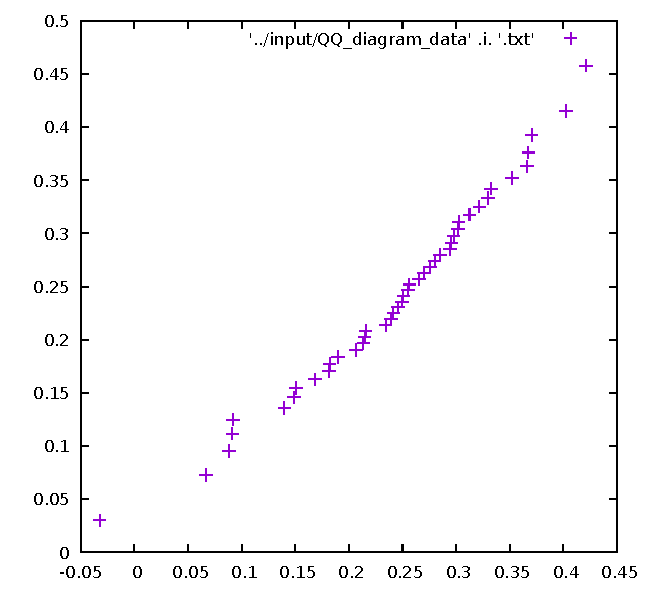
\includegraphics[width=0.3\textwidth]{../PCA/gnuplot/results_qq_diagrams/QQ_diagram4.pdf}}
  \qquad
  \subfloat[Länge der Hand]{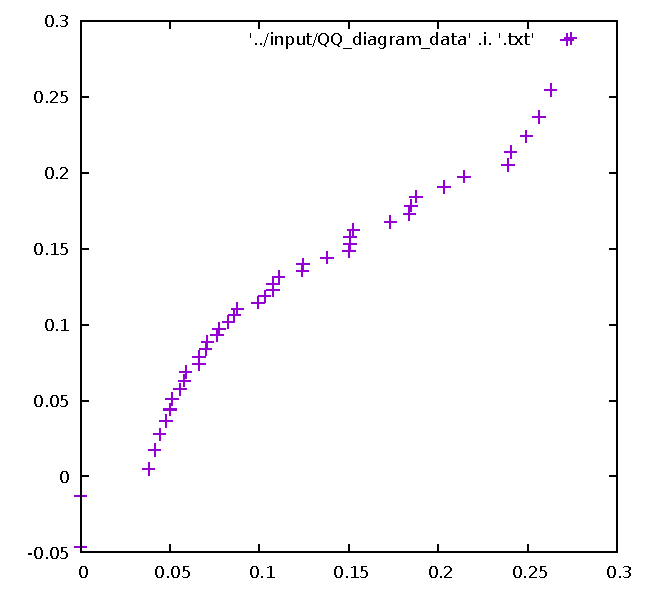
\includegraphics[width=0.3\textwidth]{../PCA/gnuplot/results_qq_diagrams/QQ_diagram24.pdf}}
  \qquad
  \subfloat[Länge des Oberschenkels]{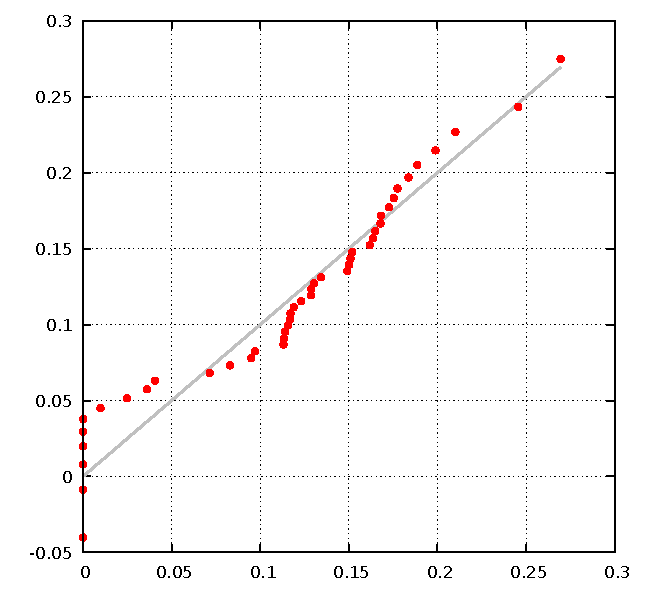
\includegraphics[width=0.3\textwidth]{../PCA/gnuplot/results_qq_diagrams/QQ_diagram25.pdf}}
  
  \caption{Beispielhaft ausgewählte Quantil-Quantil-Diagramme von drei Eingabedimensionen. (a) weicht nicht stark von der Normalverteilung ab, (b) und (c) hingegen schon mehr, sind aber trotzdem noch akzeptabel verteilt.}
  \label{qqdiagram_examples}
 \end{figure}
 
 \begin{figure}
  \subfloat[Gewicht linear]{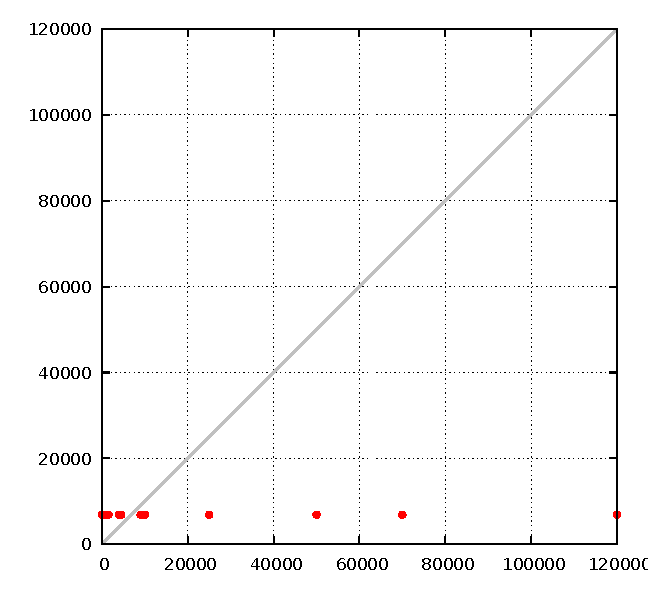
\includegraphics[width=0.3\textwidth]{../PCA/gnuplot/results_qq_diagrams/QQ_diagram_linear_weight.pdf}}
  \qquad
  \subfloat[Gewicht linear (Ausschnitt)]{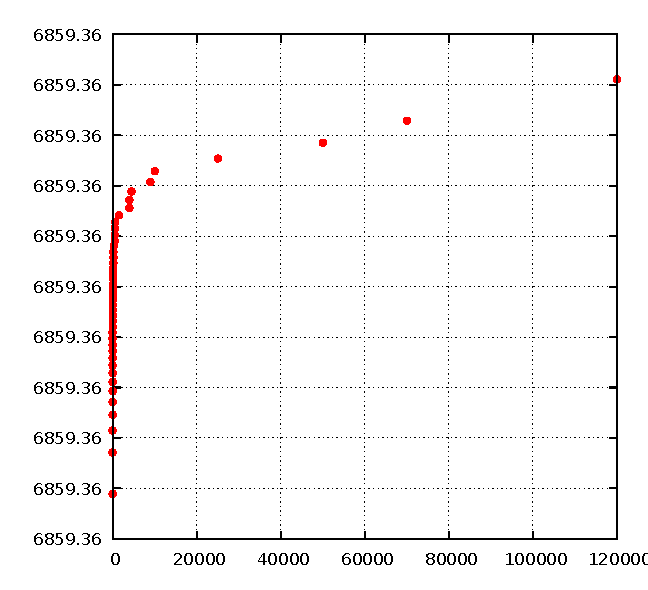
\includegraphics[width=0.3\textwidth]{../PCA/gnuplot/results_qq_diagrams/QQ_diagram_linear_weight_without_diagonal.pdf}}
  \qquad
  \subfloat[Gewicht logarithmisch]{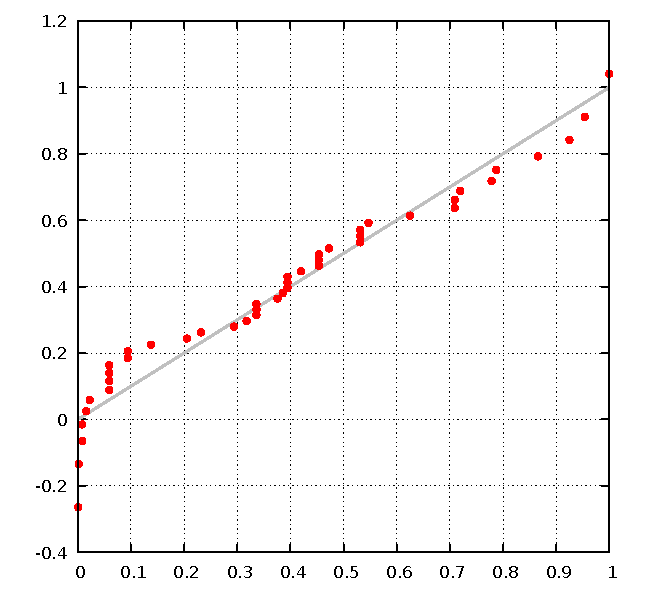
\includegraphics[width=0.3\textwidth]{../PCA/gnuplot/results_qq_diagrams/QQ_diagram28.pdf}}
  
  \caption{ Quantil-Quantil-Diagramme des Gewichts, einmal linear (a,b) und einmal mit logarithmischer Skala (c)}
  \label{qqdiagrams_weight}
 \end{figure}
 
 
 \paragraph{Skalierung der Merkmale}
 % Gewichtung der Daten
 Generell bewirkt die Skalierung eines Merkmals eine Gewichtung, denn durch eine Skalierung ändert sich die (Ko-)Varianz und somit auch die Kovarianzmatrix. Seien beispielsweise $s,t \in \mathbb{R}$, dann bewirkt eine Skalierung des Merkmals $x$ mit $s$ und eine Skalierung des Merkmals $y$ mit $t$ eine Skalierung von $s \cdot t$ der Kovarianz Cov$(x,y)$ von $x$ mit $y$, da $\mathrm{Cov}(sx, ty) = (sx - s\mu_x) (ty - t\mu_y) = st \cdot \mathrm{Cov}(x,y)$, mit Erwartungswert $\mu_i$ für \mbox{Merkmal $i$}.
 
 Wie genau werden die einzelnen Merkmale nun skaliert?
 
 % Bildkoordinaten + -längen
 Zunächst werden alle Merkmale auf das Intervall $[0, 1]$ skaliert, damit alle den gleichen Einfluss haben.
 Bei Koordinaten oder Längen im Bild bedeutet das, dass sie durch $1000$ geteilt werden, da sie in Pixeln dargestellt werden und das Bild eine Größe von $1000 \times 1000$ Pixeln hat. Bei Längen von Strecken im Bild wären dabei theoretisch auch Werte größer $1000$px möglich. Solche Längen wären aber unrealistisch und werden deshalb ignoriert.\\
 Koordinaten und Längen im Bild sind diejenigen Merkmale, die hier am interessantesten sind. Sie stellen den Verlauf der Wirbelsäule und die Längen der Knochen der Extremitäten dar. Deshalb sollten sie den größten Einfluss auf die Hauptkomponenten der PCA haben. Alle anderen Merkmale werden kleiner skaliert.
 
 % Merkmale nach angenommenem Maximum skalieren?
 Man könnte statt einer Skalierung mit $0.001$ auch für jedes einzelne Merkmal den maximal und minimal angenommenen Wert ermitteln und sie dann so skalieren, dass sie Intervalle gleicher Länge abdecken. Das würde ausgleichen, dass \zb kleine Längen eine kleinere Varianz und damit auch einen kleineren Einfluss haben.
 Da aber kleine Elemente im Bild auch weniger zum Gesamteindruck beitragen, wirkt es natürlich, dass sie auch weniger Einfluss auf die Hauptkomponenten haben.
 Deshalb wird die oben beschriebene Variante verwendet. Falls es in Zukunft Gründe für eine andere Gewichtung gäbe, ließe sich das aber leicht anpassen.
 
 % kleinskalieren von Flügeln, Beinen und Gewicht
 Die diskreten Merkmale \emph{Flügel} und \emph{Beine mit Bodenkontakt} und das logarithmische \emph{Gewicht} werden zunächst ebenfalls auf das Intervall $[0, 1]$ skaliert. Das bedeutet für das angepasste Gewicht $\bar{w} = \frac{\mathrm{log}(w+1)}{\mathrm{log}(\mathrm{max}+1)}$. Das schwerste Wirbeltier ist der Blauwal mit 120 Tonnen (siehe Abschnitt \ref{bigAndSmall}). Deshalb ist hier max $= 120.000$kg.\\
 Danach werden die Werte noch einmal durch $100$ geteilt, um ihren Einfluss zu verringern. Das Ziel ist, dass diese Merkmale nicht als große Einträge in den größten Eigenvektoren (den Hauptkomponenten) auftauchen. Ohne diese Skalierung sind diese Merkmale recht dominant. Mit der Skalierung hingegen sind sie in den größten Eigenvektoren unter den kleinsten Werten zu finden.\\
 Obwohl die Merkmale nun sehr kleine Werte annehmen, sind ihre Korrelationen mit anderen Merkmalen trotzdem noch vorhanden. Wird ein zufälliger $n$-dimensionaler \mbox{Punkt $p$} mit der gegebenen Normalverteilung generiert, so enthält er also trotzdem Informationen zu \emph{Flügeln} und \emph{Beinen mit Bodenkontakt}. Erst wenn $p$ auf seine Hauptkomponenten reduziert wird, fallen die meisten Informationen dazu weg.
 
 % Projektion auf Eigenvektoren
 Interessant ist die Projektion der Eingabedaten auf die größten beiden  Eigenvektoren. In Abbildung \ref{projections_scales} ist gut zu vergleichen was die Effekte der Skalierung der Eingabedaten sind. Ganz links sind die Ergebnisse zu sehen, die entstehen, wenn alle Merkmale nur auf das Intervall $[0, 1]$ skaliert werden. In der Mitte geht das Gewicht nicht mehr linear, sondern logarithmisch ein und ganz rechts sind \emph{Flügel}, \emph{Anzahl Beine} und \emph{Gewicht} zusätzlich klein skaliert. Gut zu sehen ist, wie sich die Clusterbildung durch die Skalierung verringert. Gibt es weniger Cluster, ist die Verteilung der Daten näher an einer Normalverteilung.
 
 % Projektion unterschiedlich gelabelt
 In Abbildung \ref{projections_tags} ist noch einmal jeweils die Projektion der skalierten Daten auf die ersten beiden Eigenvektoren zu sehen. Diesmal sind die Daten anhand der verschiedenen diskret erhobenen Merkmale markiert. Es ist \zb schön zu sehen, dass alle Tiere mit Flügeln auch Vögel sind und dass fast alle Tiere, die zwei Beine haben, Vögel sind. Vier Tiere haben zwei Beine, sind aber keine Vögel: Ohrenrobbe, Seehund, Tyrannosaurus Rex und Känguru.

 \begin{figure}
  \subfloat[gleiche Skalierung aller Dimensionen]{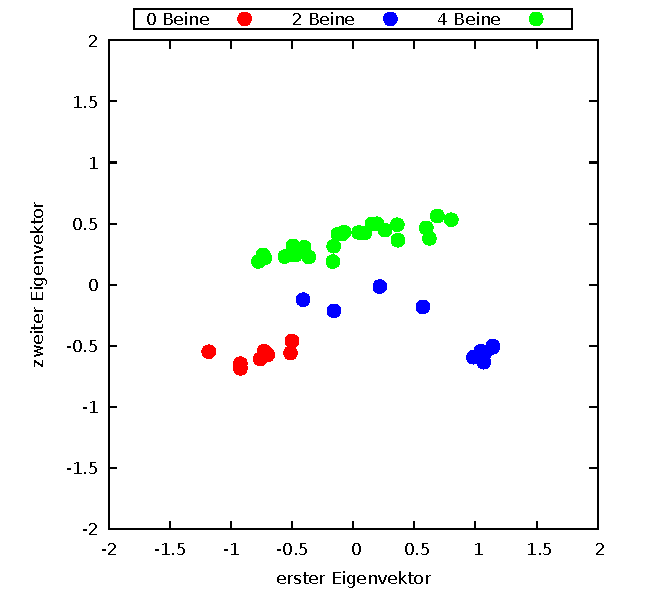
\includegraphics[width=0.3\textwidth]{../PCA/gnuplot/results_with_leg_tag/projection_eigenvectors12.pdf}}
  \qquad
  \subfloat[logarithmisches Gewicht]{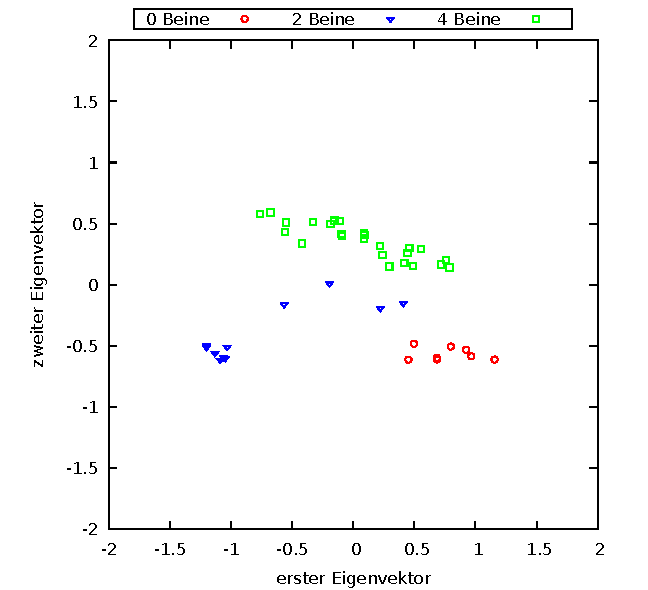
\includegraphics[width=0.3\textwidth]{../PCA/gnuplot_log_weight/results_with_leg_tag/projection_eigenvectors12.pdf}}
  \qquad
  \subfloat[skalierte "`Zusatzmerkmale"']{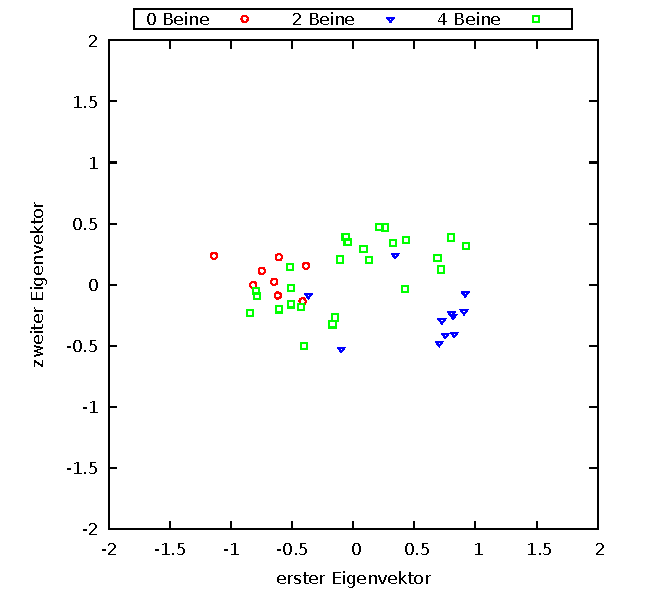
\includegraphics[width=0.3\textwidth]{../PCA/gnuplot_log_weight_with_downscaled_wings_legs_and_weight/results_with_leg_tag/projection_eigenvectors12.pdf}}
  
  \caption{Dargestellt sind hier jeweils die Projektionen der Eingabedaten auf die ersten beiden Eigenvektoren. Für jede Version wurden die Eingabedaten unterschiedlich vorverarbeitet. (a) Skalierung aller erhobenen Daten auf das Intervall $[0, 1]$, (b) zusätzlich Verwendung von logarithmischem Gewicht, statt linearem, (c) zusätzliche Skalierung der Merkmale \emph{Flügel}, \emph{Anzahl Beine} und \emph{Gewicht} mit $0,01$.}
  \label{projections_scales}
 \end{figure}
 
 \begin{figure}
  \subfloat[Flügel]{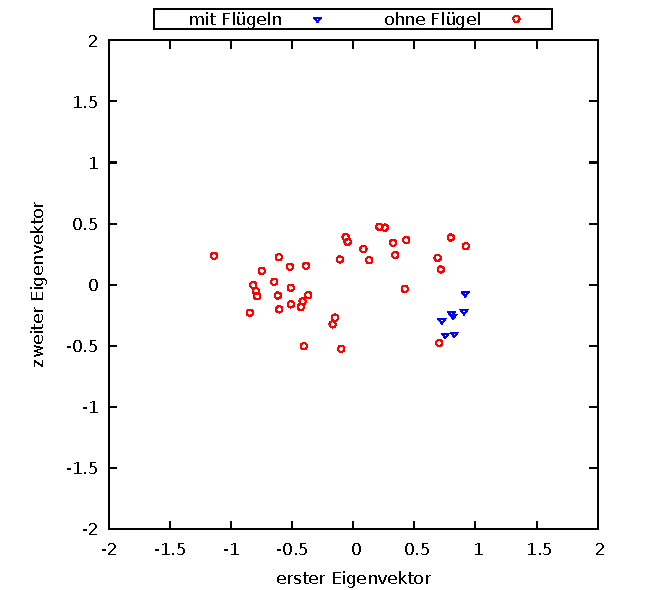
\includegraphics[width=0.3\textwidth]{../PCA/gnuplot_log_weight_with_downscaled_wings_legs_and_weight/results_with_wing_tag/projection_eigenvectors12.pdf}}
  \qquad
  \subfloat[Anzahl Beine mit Bodenkontakt]{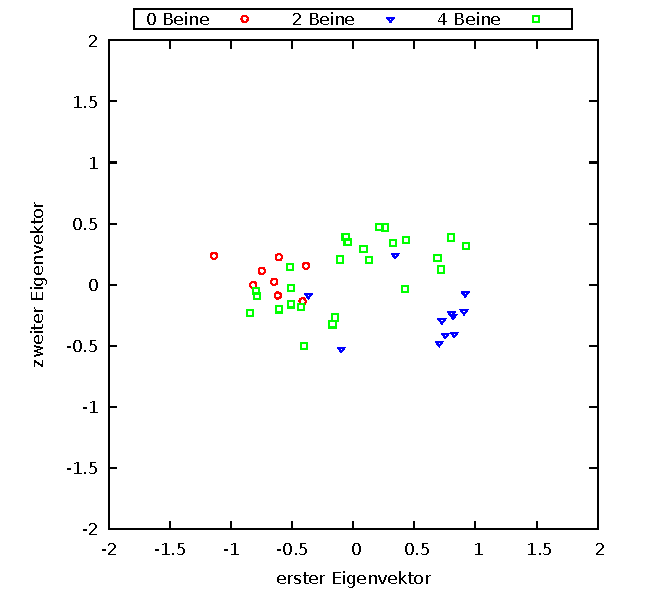
\includegraphics[width=0.3\textwidth]{../PCA/gnuplot_log_weight_with_downscaled_wings_legs_and_weight/results_with_leg_tag/projection_eigenvectors12.pdf}}
  \qquad
  \subfloat[Tierklasse]{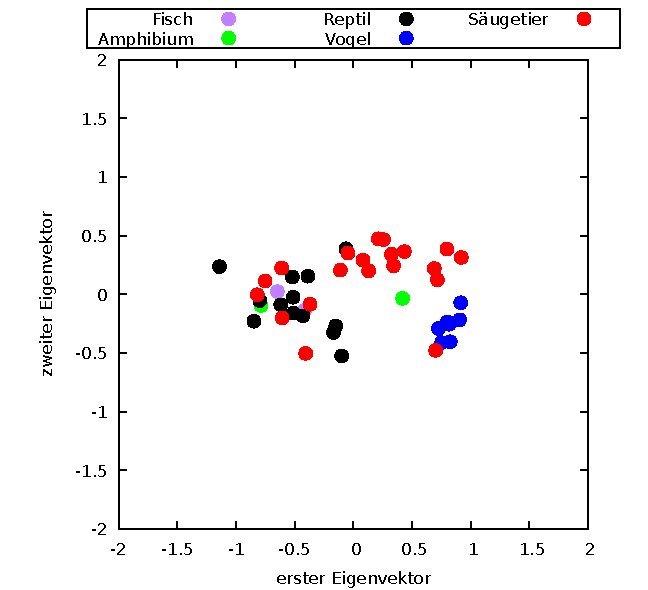
\includegraphics[width=0.3\textwidth]{../PCA/gnuplot_log_weight_with_downscaled_wings_legs_and_weight/results_with_animal_class_tag/projection_eigenvectors12.pdf}}
  
  \caption{Projektion der, wie in Abbildung \ref{projections_scales}c skalierten, Eingabedaten auf die Ebene, die durch den ersten und zweiten Eigenvektor aufgespannt wird. Markiert sind jeweils ob Flügel vorhanden sind (a), die Anzahl der Beinpaare (b) und die \mbox{Tierklasse (c)}.}
  \label{projections_tags}
 \end{figure}
 
 
 % Ergebnis wieder normalverteilt
 Auch im Koordinatensystem der Eigenvektoren sollten die Daten wieder normalverteilt sein. Dies wurde ebenfalls mit Quantil-Quantil-Diagrammen untersucht. In \mbox{Abbildung \ref{qqdiagram_projections}} sind die Ergebnisse für die ersten drei Eigenvektoren zu sehen. Es gibt, wie bei den Eingabedaten, keine allzu großen Abweichungen.
 
 \begin{figure}
  \subfloat[erster Eigenvektor]{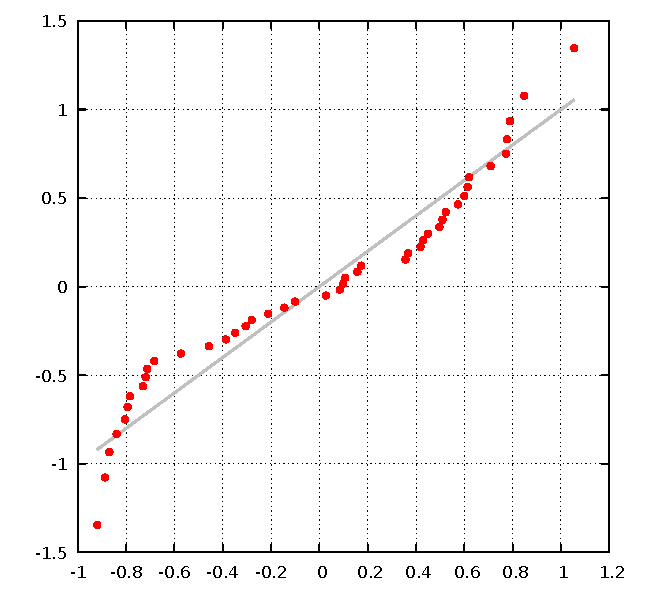
\includegraphics[width=0.3\textwidth]{../PCA/gnuplot_log_weight_with_downscaled_wings_legs_and_weight/results_qqdiagrams/QQ_diagram_projection0.pdf}}
  \qquad
  \subfloat[zweiter Eigenvektor]{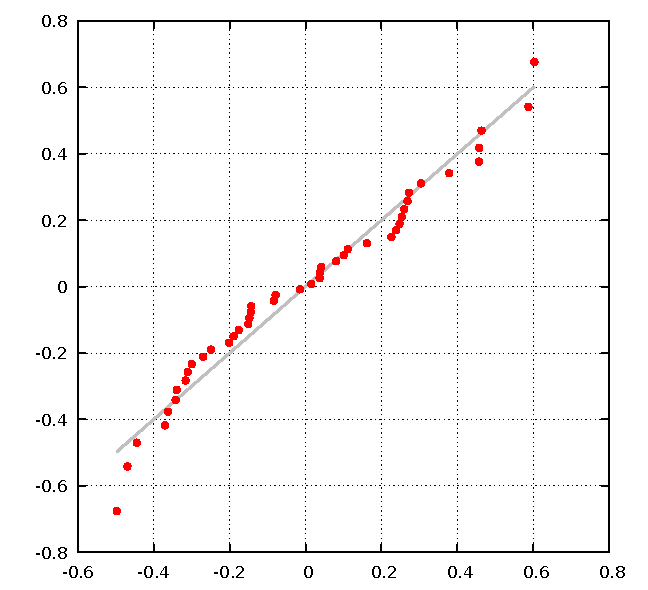
\includegraphics[width=0.3\textwidth]{../PCA/gnuplot_log_weight_with_downscaled_wings_legs_and_weight/results_qqdiagrams/QQ_diagram_projection1.pdf}}
  \qquad
  \subfloat[dritter Eigenvektor]{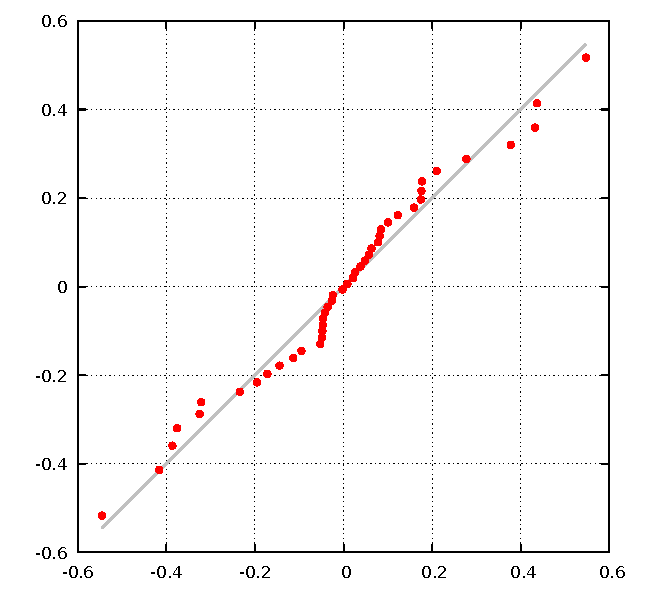
\includegraphics[width=0.3\textwidth]{../PCA/gnuplot_log_weight_with_downscaled_wings_legs_and_weight/results_qqdiagrams/QQ_diagram_projection2.pdf}}
  
  \caption{Quantil-Quantil-Diagramme der Eingabedaten projiziert auf die größten drei Eigenvektoren.}
  \label{qqdiagram_projections}
 \end{figure}
 
 
 \paragraph{Spezielle Punkte}
 % Mittelwert
 Der Mittelwert der skalierten Eingabedaten ist in Abbildung \ref{mean} visualisiert.
 Wie auch bei der Datenerhebung ist hier die Position der Wirbelsäule in einem $1000 \times 1000$ Pixel Bild gezeigt. Da von den Knochen der Vorder- und Hinterextremitäten nur die Längen erhoben wurden, sind ihre Positionen nicht realistisch. Die restlichen Daten sind nicht visualisiert, sondern nur in Textform angegeben.
 
 \begin{figure}
  \centering
  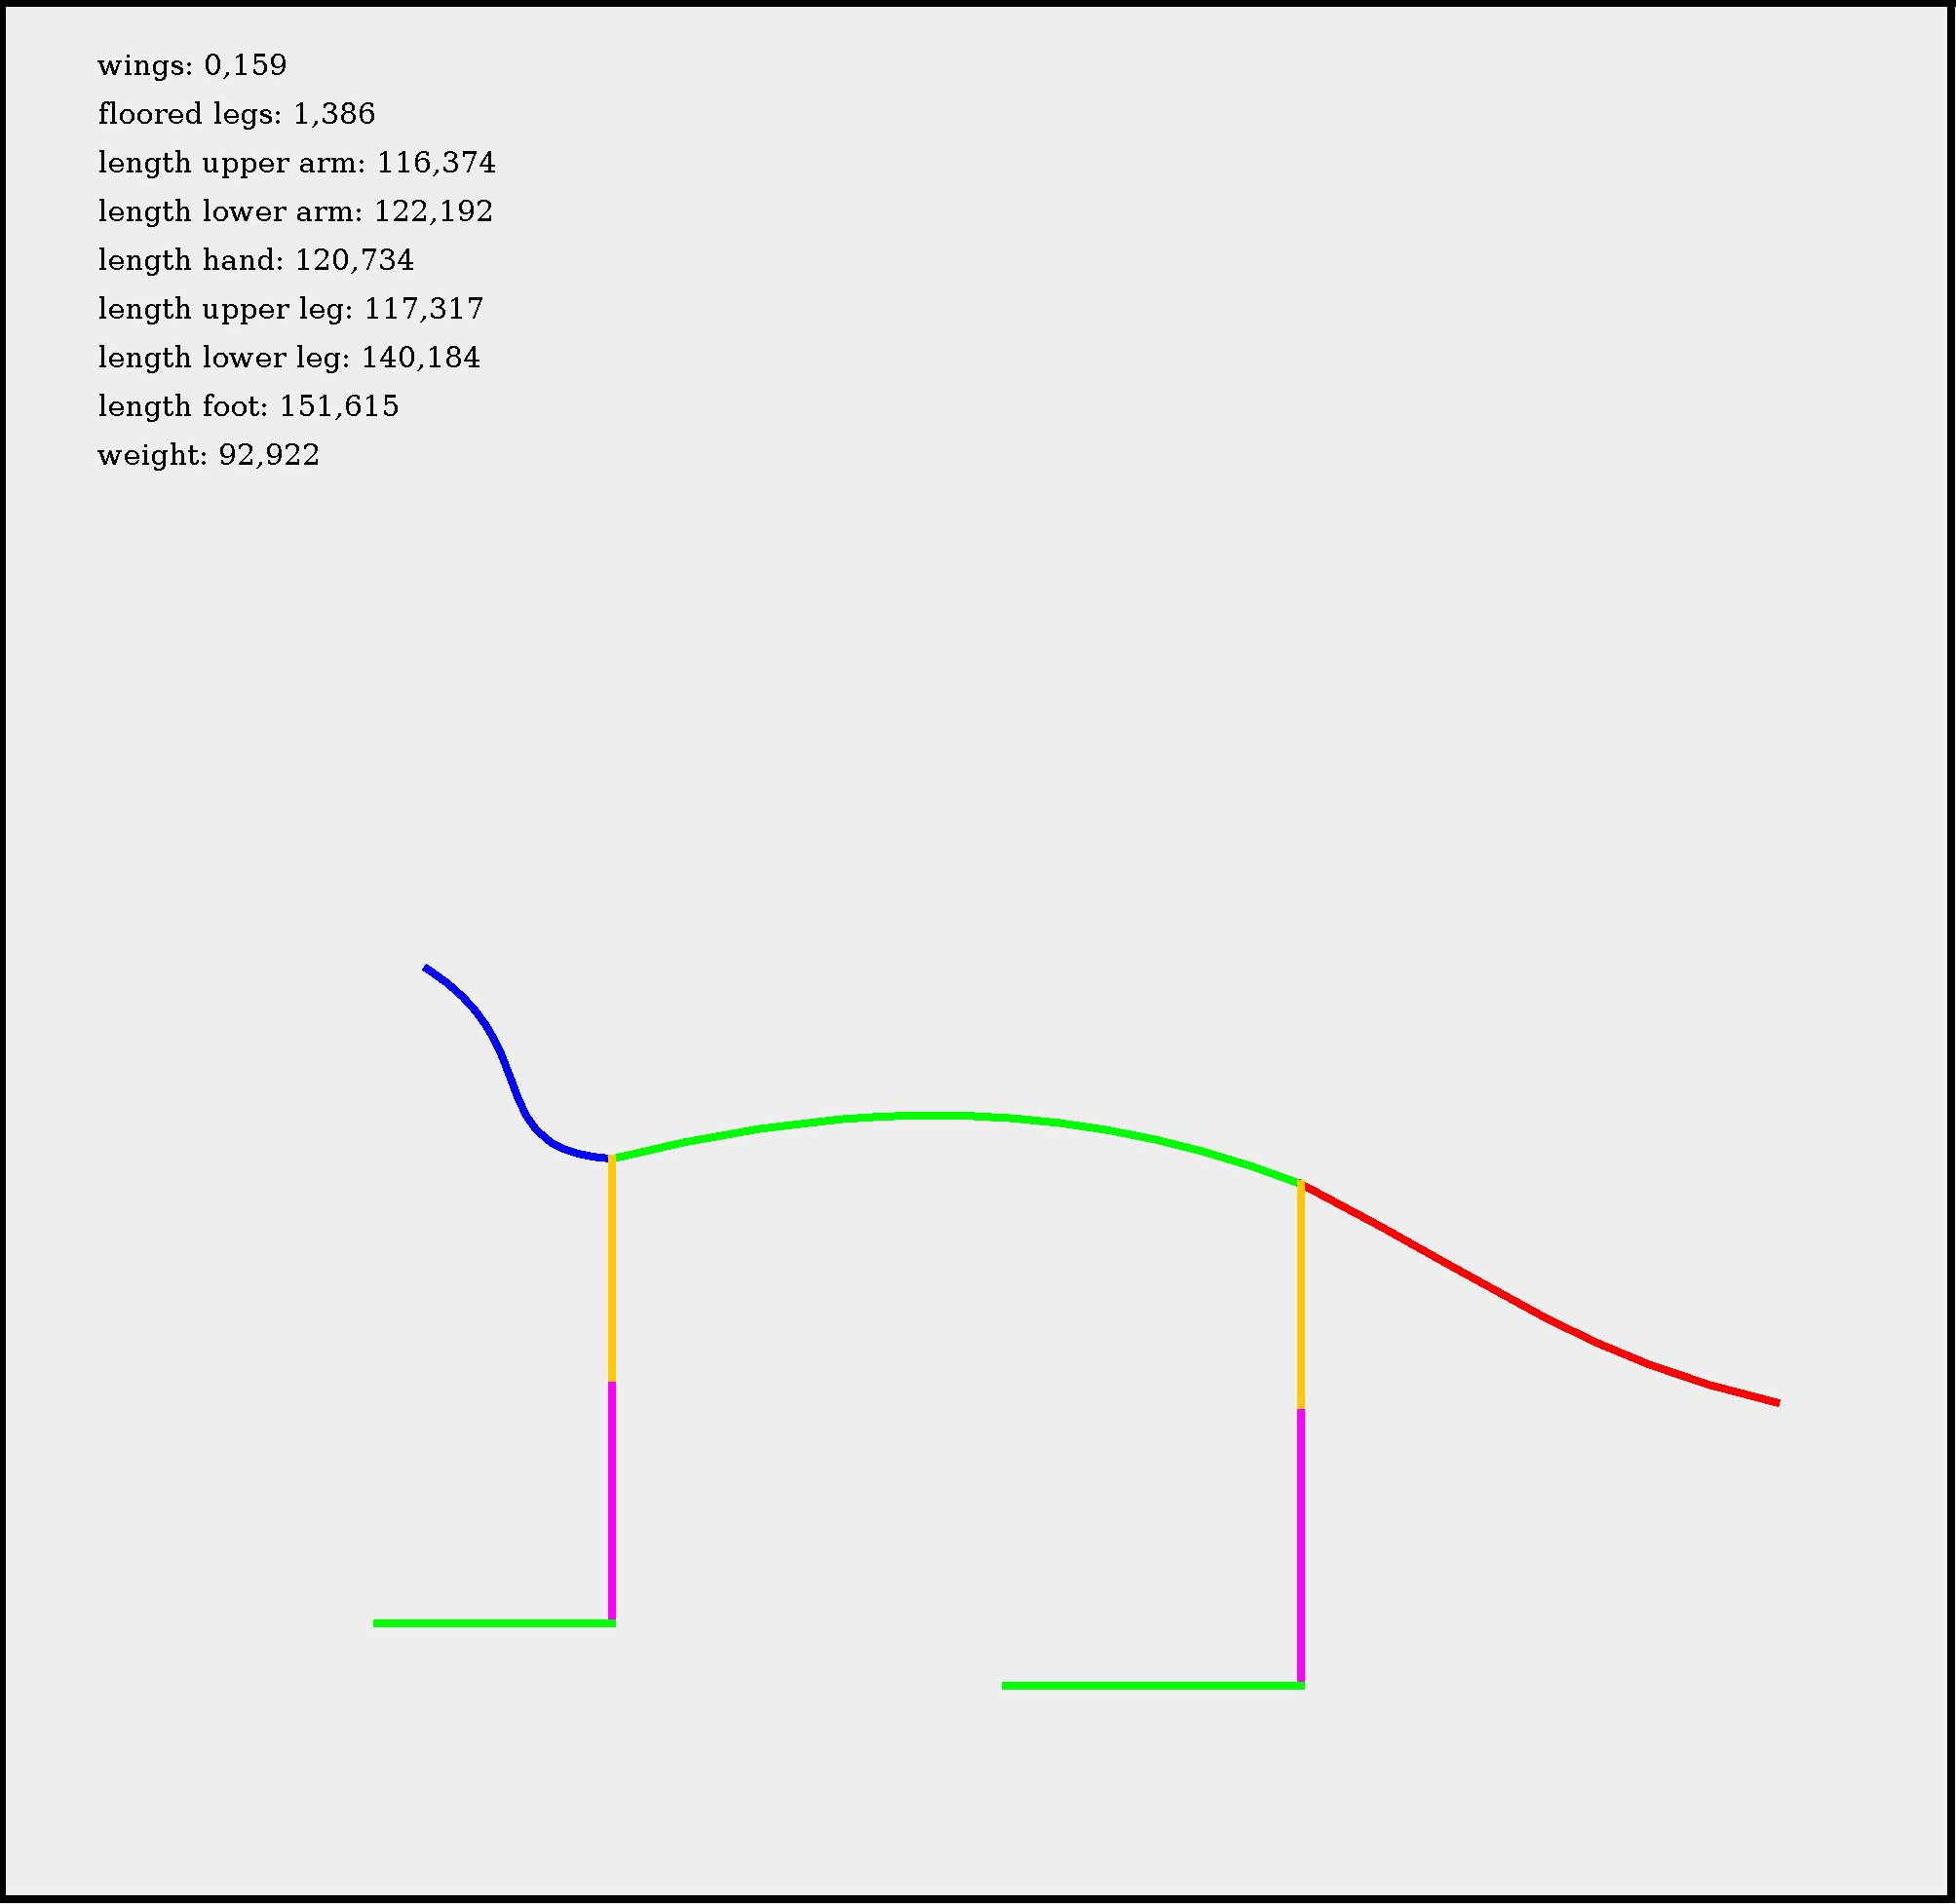
\includegraphics[width=0.5\textwidth]{../PCA/mean_log_weight_downscaled_wings_legs_and_weight(onlyBox,stroke4).jpg}
  \caption{Visualisierung des Mittelwerts der skalierten Eingabedaten. Die Werte, die nicht grafisch visualisiert sind, sind folgende: \emph{Flügel} $0{,}159$, \emph{Beine mit Bodenkontakt} $1{,}39$, \emph{Gewicht} $93$kg.}
  \label{mean}
 \end{figure}
 
 % min Abstand
 Den minimalen Abstand zum Mittelwert hat der Klippschliefer (siehe Abbildung \ref{klippschliefer_farbig}). Zusätzlich zum Bild wurde für den Klippschliefer folgende Daten erhoben:
 \emph{Tierklasse} Säugetier, \emph{Flügel} nein, \emph{Beine mit Bodenkontakt} $2$, \emph{Gewicht} $4$kg.
 
 % max Abstand
 Den maximalen Abstand hat die Schlange. Die erhobenen Daten sind hier:
 \emph{Tierklasse} Reptil, \emph{Flügel} nein, \emph{Beine mit Bodenkontakt} $0$, \emph{Gewicht} $50$kg.
 Die Schlange ist allerdings das einzige Tier zu dem es kein "`echtes"' Bild des Skeletts gibt. Das liegt daran, dass es keine seitlichen Abbildungen von ausgestreckten Schlangen gibt. Sie werden eigentlich immer gekrümmt dargestellt, da sonst das Bild sehr lang und schmal werden würde. 
 Da aber versucht wurde, eine möglichst große Variation an Skeletten zu erheben, und ein Schlangenskelett, in der hier nötigen Auflösung, sehr einfach darzustellen ist, wurde trotzdem ein Bild erstellt. Dieses Bild enthält nur eine horizontale Linie knapp über dem unteren Bildrand, die den Rücken darstellen soll. Extremitäten und ersichtliche Punkte, an denen der Rücken in Hals oder Schwanz übergeht, gibt es bei Schlangen nicht.
 
 % zweitgrößter Abstand (da max Schlange)
 Der Punkt mit dem zweitgrößten Abstand zum Mittelwert ist das Känguru (siehe Abbildung \ref{kaenguru_farbig}). Zusätzlich zum Bild gibt es hier folgende Daten:
  \emph{Tierklasse} Säugetier, \emph{Flügel} nein, \emph{Beine mit Bodenkontakt} $1$, \emph{Gewicht} $50$kg
  
 \begin{figure}[ht]
  \subfloat[Klippschliefer]{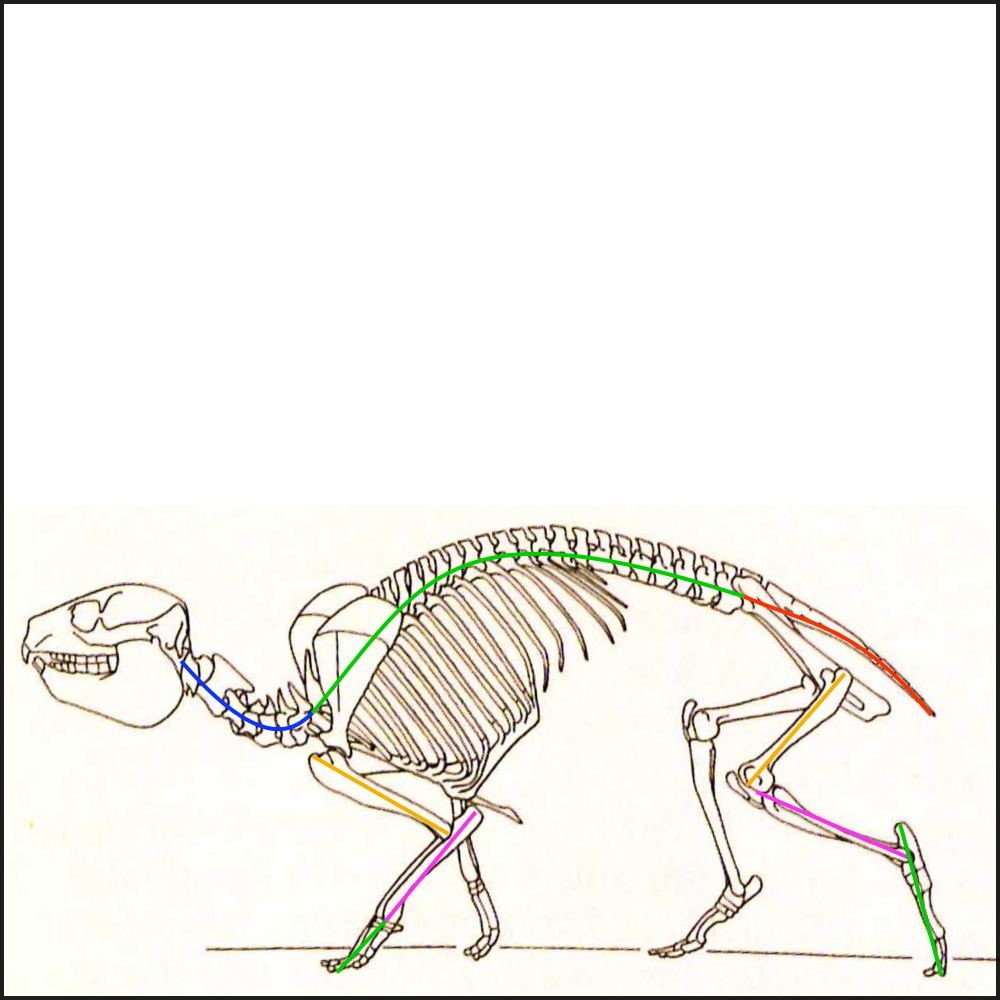
\includegraphics[width=0.5\textwidth]{../PCA/Skelettbilder/Klippschliefer_farbig.png} \label{klippschliefer_farbig}}
  \qquad
  \subfloat[Känguru]{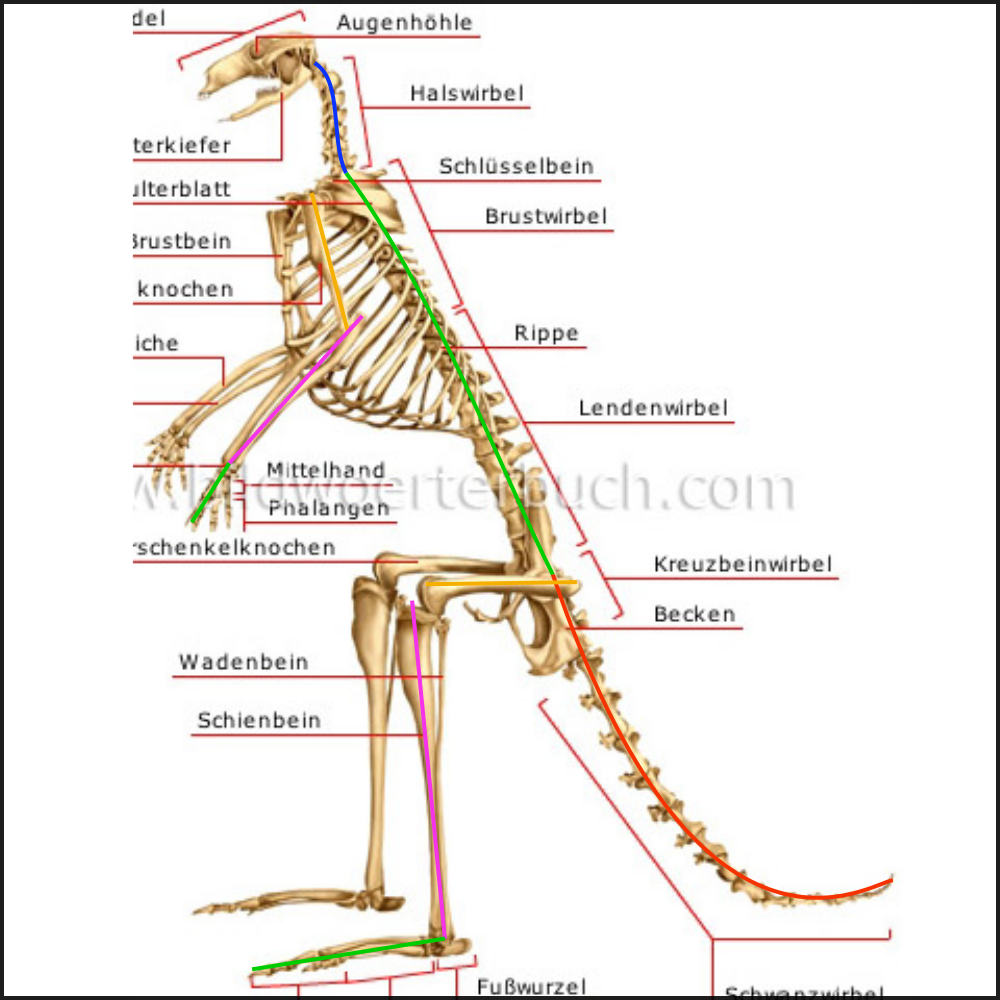
\includegraphics[width=0.5\textwidth]{../PCA/Skelettbilder/Kaenguru_farbig.png}\label{kaenguru_farbig}}
  
  \caption{Annotierte Bild des Skeletts eines Klippschliefers (a) und eines \mbox{Kängurus (b)}. Die Teile der Wirbelsäule und die Knochen der Extremitäten sind hier jeweils mit der gleichen Farbe markiert wie in der Visualisierung des Mittelwerts (Abbildung \ref{mean})}
 \end{figure}
 

 \newpage
 %-----------------------------------
 \section{Analyse der Ergebnisse}
 \label{section_pca_result_analysis}
 
 % Eigenvektoren und Rekonstruktionen
 Zu $29$ Eingabedimensionen gibt es auch $29$ Eigenvektoren mit Eigenwerten größer $0$. Der kleinste Eigenwert ist $0{,}000001$. Von den Eigenwerten sind $7$ größer als $0{,}01$. 
 
 Die Eigenwerte $\lambda_i$ geben die Varianz der Normalverteilung entlang der Achse des zugehörigen Eigenvektors $v_i$ an. Die Summe aller Varianzen $\Sigma_{i=0}^n \lambda_i$ ist ein Maß für den Informationsgehalt. Werden alle Eigenvektoren verwendet um die Daten darzustellen, so ist $100\%$ der Information vorhanden, bei $m \le n$ Eigenvektoren jeweils der Anteil $\Sigma_{i=0}^m \lambda_i / \Sigma_{i=0}^n \lambda_i$.\\
 Die ersten $6$ Eigenvektoren enthalten $92{,}2\%$ der Informationen, die ersten $10$ enthalten $96{,}9\%$ und die ersten $20$ enthalten $99{,}8\%$.
 
 Versucht man die Eingabedaten durch die Eigenvektoren mit den größten Eigenwerten anzunähern, so funktioniert das bei manchen Tieren ganz gut, wie \zb beim Archaeopteryx (siehe Abbildung \ref{archaeopteryx}) schon mit den größten $6$ Eigenvektoren, bei anderen aber eher schlechter (siehe Frosch, Abbildung \ref{frosch}).\\
 Trotzdem sind die berechneten Eigenvektoren hilfreich um zufällige Punkte mit der Verteilung der Eingabebeispiele zu generieren (wie auch beschrieben in Abschnitt \ref{PCA}).
 
 \begin{figure}
  \centering
  \subfloat[Rekonstruktion aus 6 Eigenvektoren]{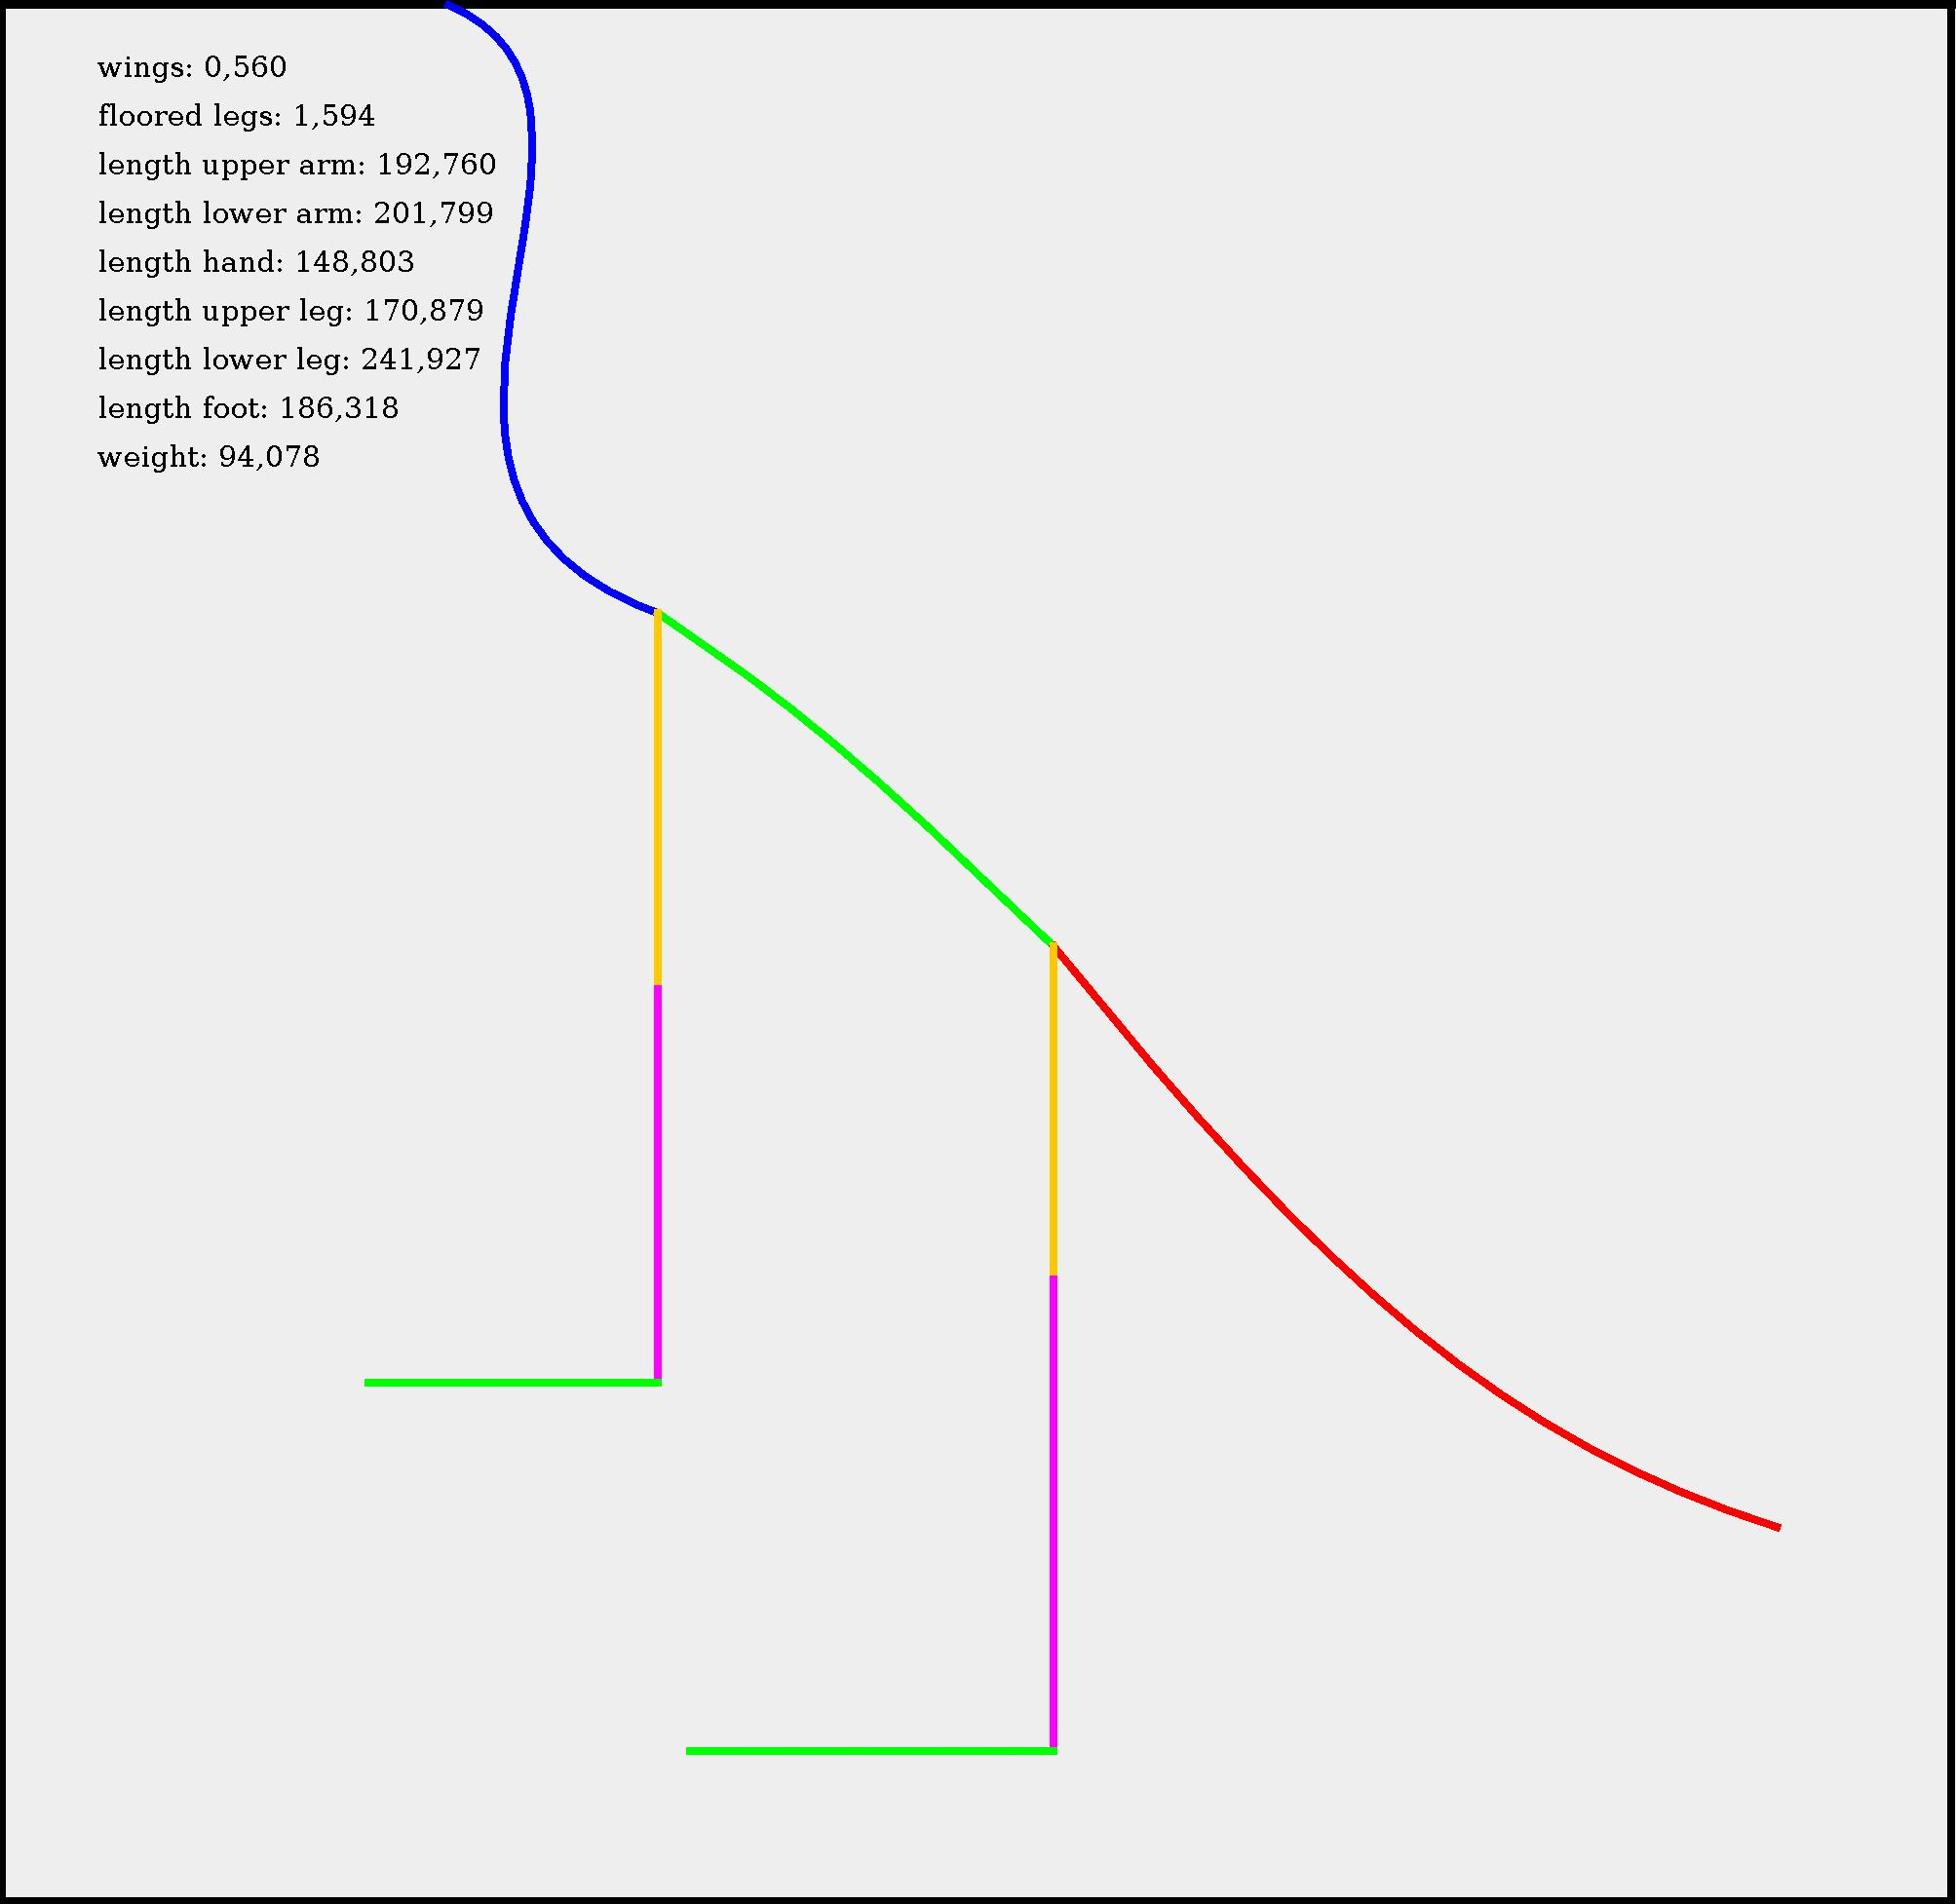
\includegraphics[width=0.4\textwidth]{../PCA/animal_reconstructions_log_weight_downscaled_wings_legs_and_weight/6EV/Archaeopteryx_Ausschnitt.jpg}}
  \qquad
  \subfloat[Eingabebild]{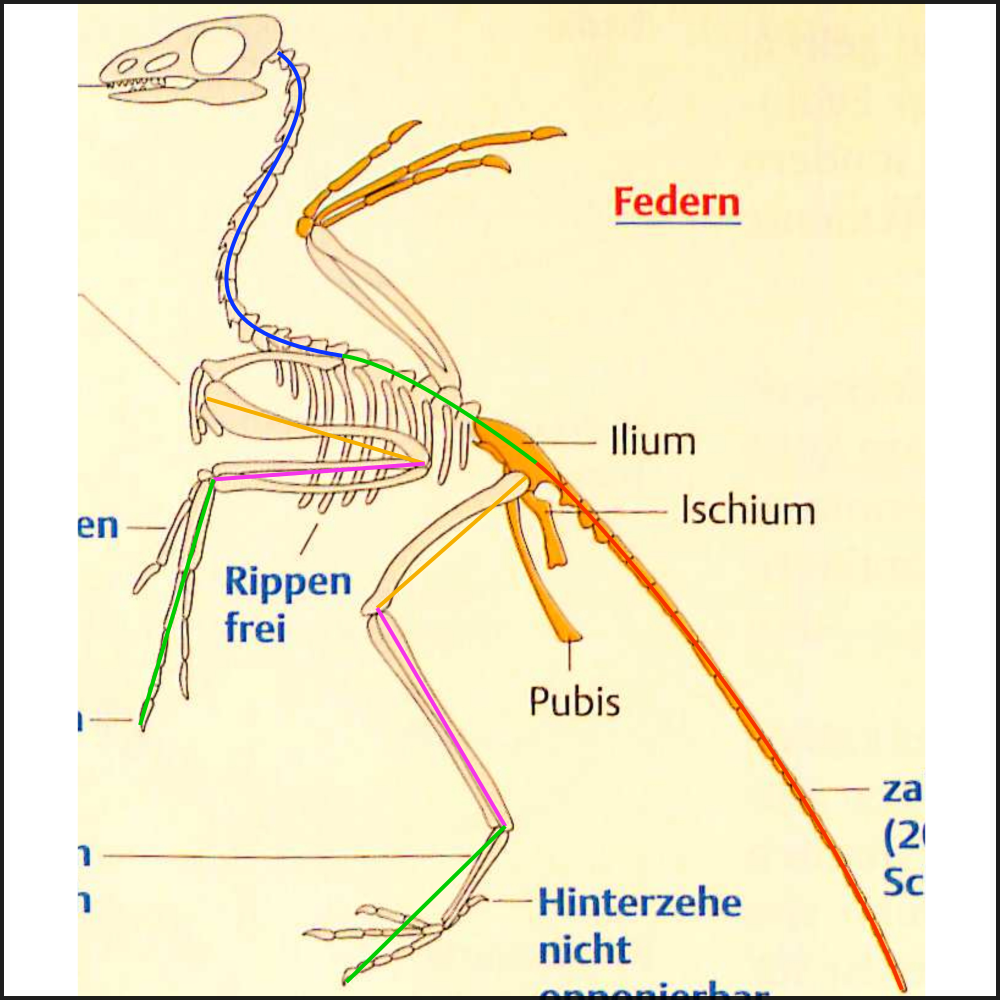
\includegraphics[width=0.4\textwidth]{../PCA/Skelettbilder/Archaeopteryx_farbig.png}}
  
  \caption{Archaeopteryx nicht visualisierte Daten der Rekonstruktion: \emph{Flügel} $0{,}56$, \emph{Beine mit Bodenkontakt} $1{,}594$, \emph{Gewicht} $94{,}1$kg, Originalwert für das \emph{Gewicht}: $1$kg}
  \label{archaeopteryx}
 \end{figure}
 
\begin{figure}
  \centering
  \subfloat[$6$ Eigenvektoren,
  \emph{Flügel} $0{,}4$, \emph{Beine mit Bodenkontakt} $1{,}27$, \emph{Gewicht} $90{,}2$kg]
  {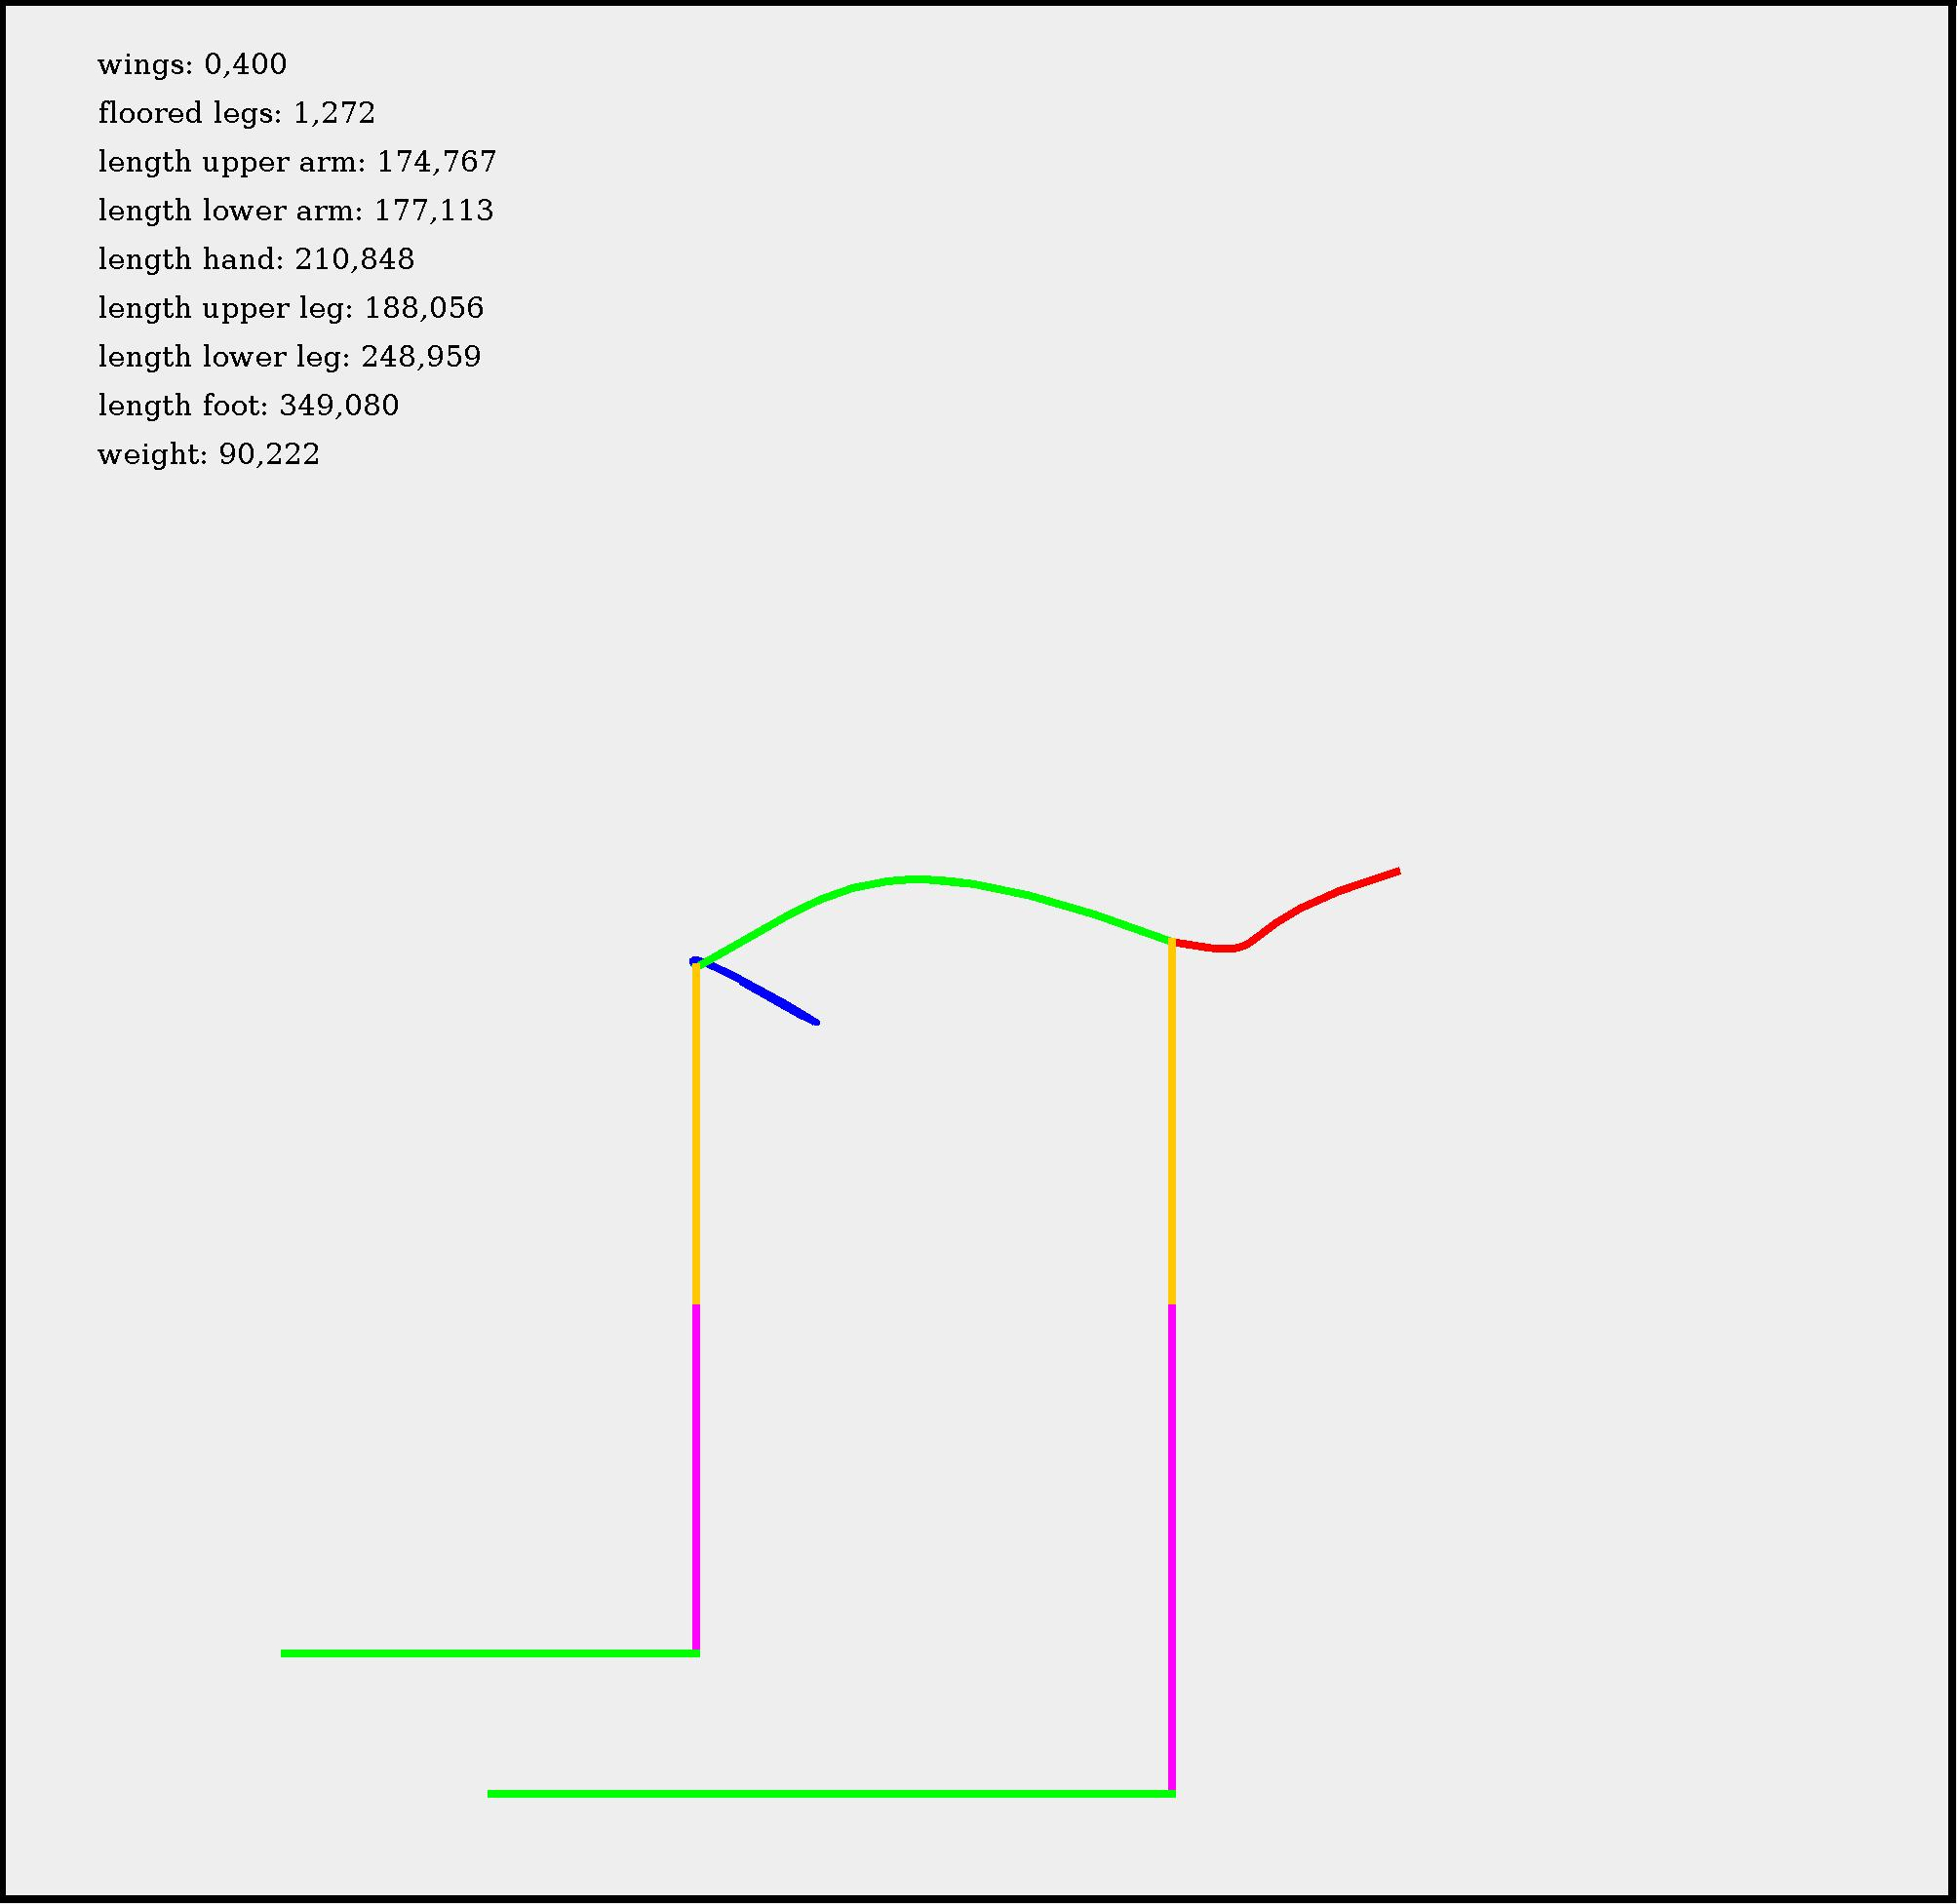
\includegraphics[width=0.4\textwidth]{../PCA/animal_reconstructions_log_weight_downscaled_wings_legs_and_weight/6EV/Frosch_Ausschnitt.jpg}}
  \qquad
  \subfloat[$10$ Eigenvektoren,
  \emph{Flügel} $0{,}151$, \emph{Beine mit Bodenkontakt} $1{,}28$, \emph{Gewicht} $88{,}7$kg]{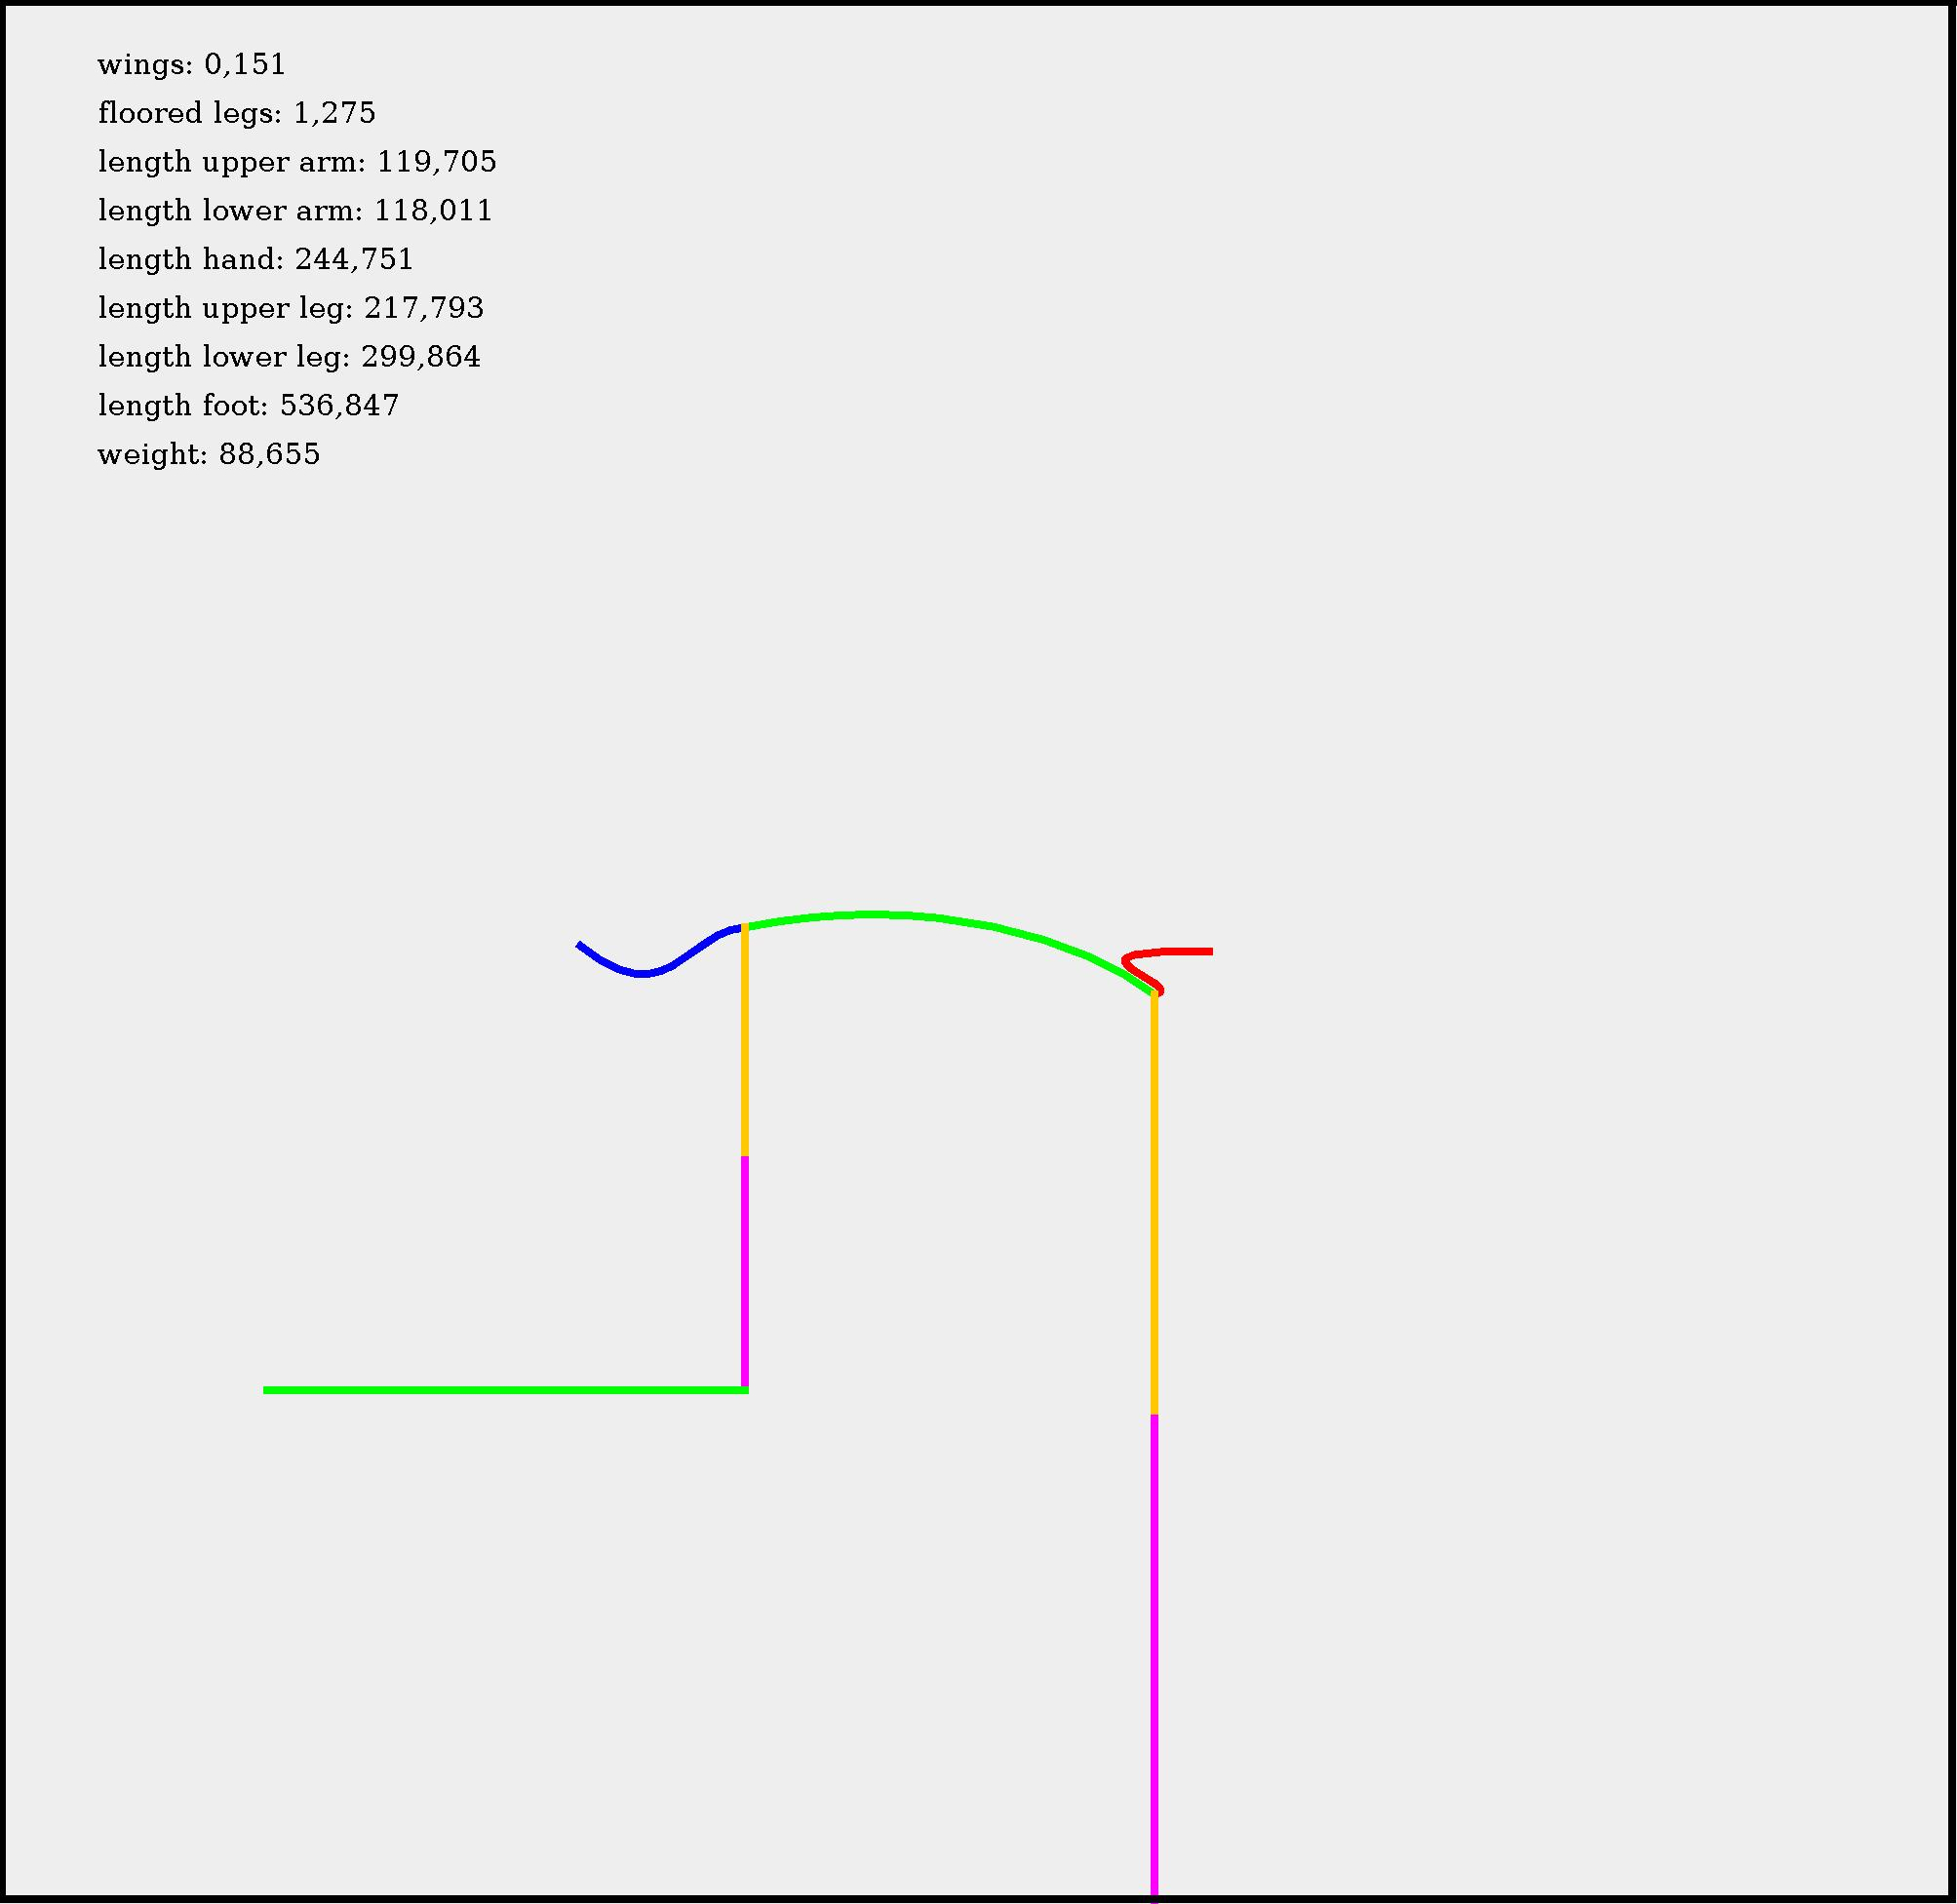
\includegraphics[width=0.4\textwidth]{../PCA/animal_reconstructions_log_weight_downscaled_wings_legs_and_weight/10EV/Frosch_Ausschnitt.jpg}}
  \\
  \subfloat[$20$ Eigenvektoren,
  \emph{Flügel} $0{,}217$, \emph{Beine mit Bodenkontakt} $1{,}7$, \emph{Gewicht} $89{,}2$kg]
  {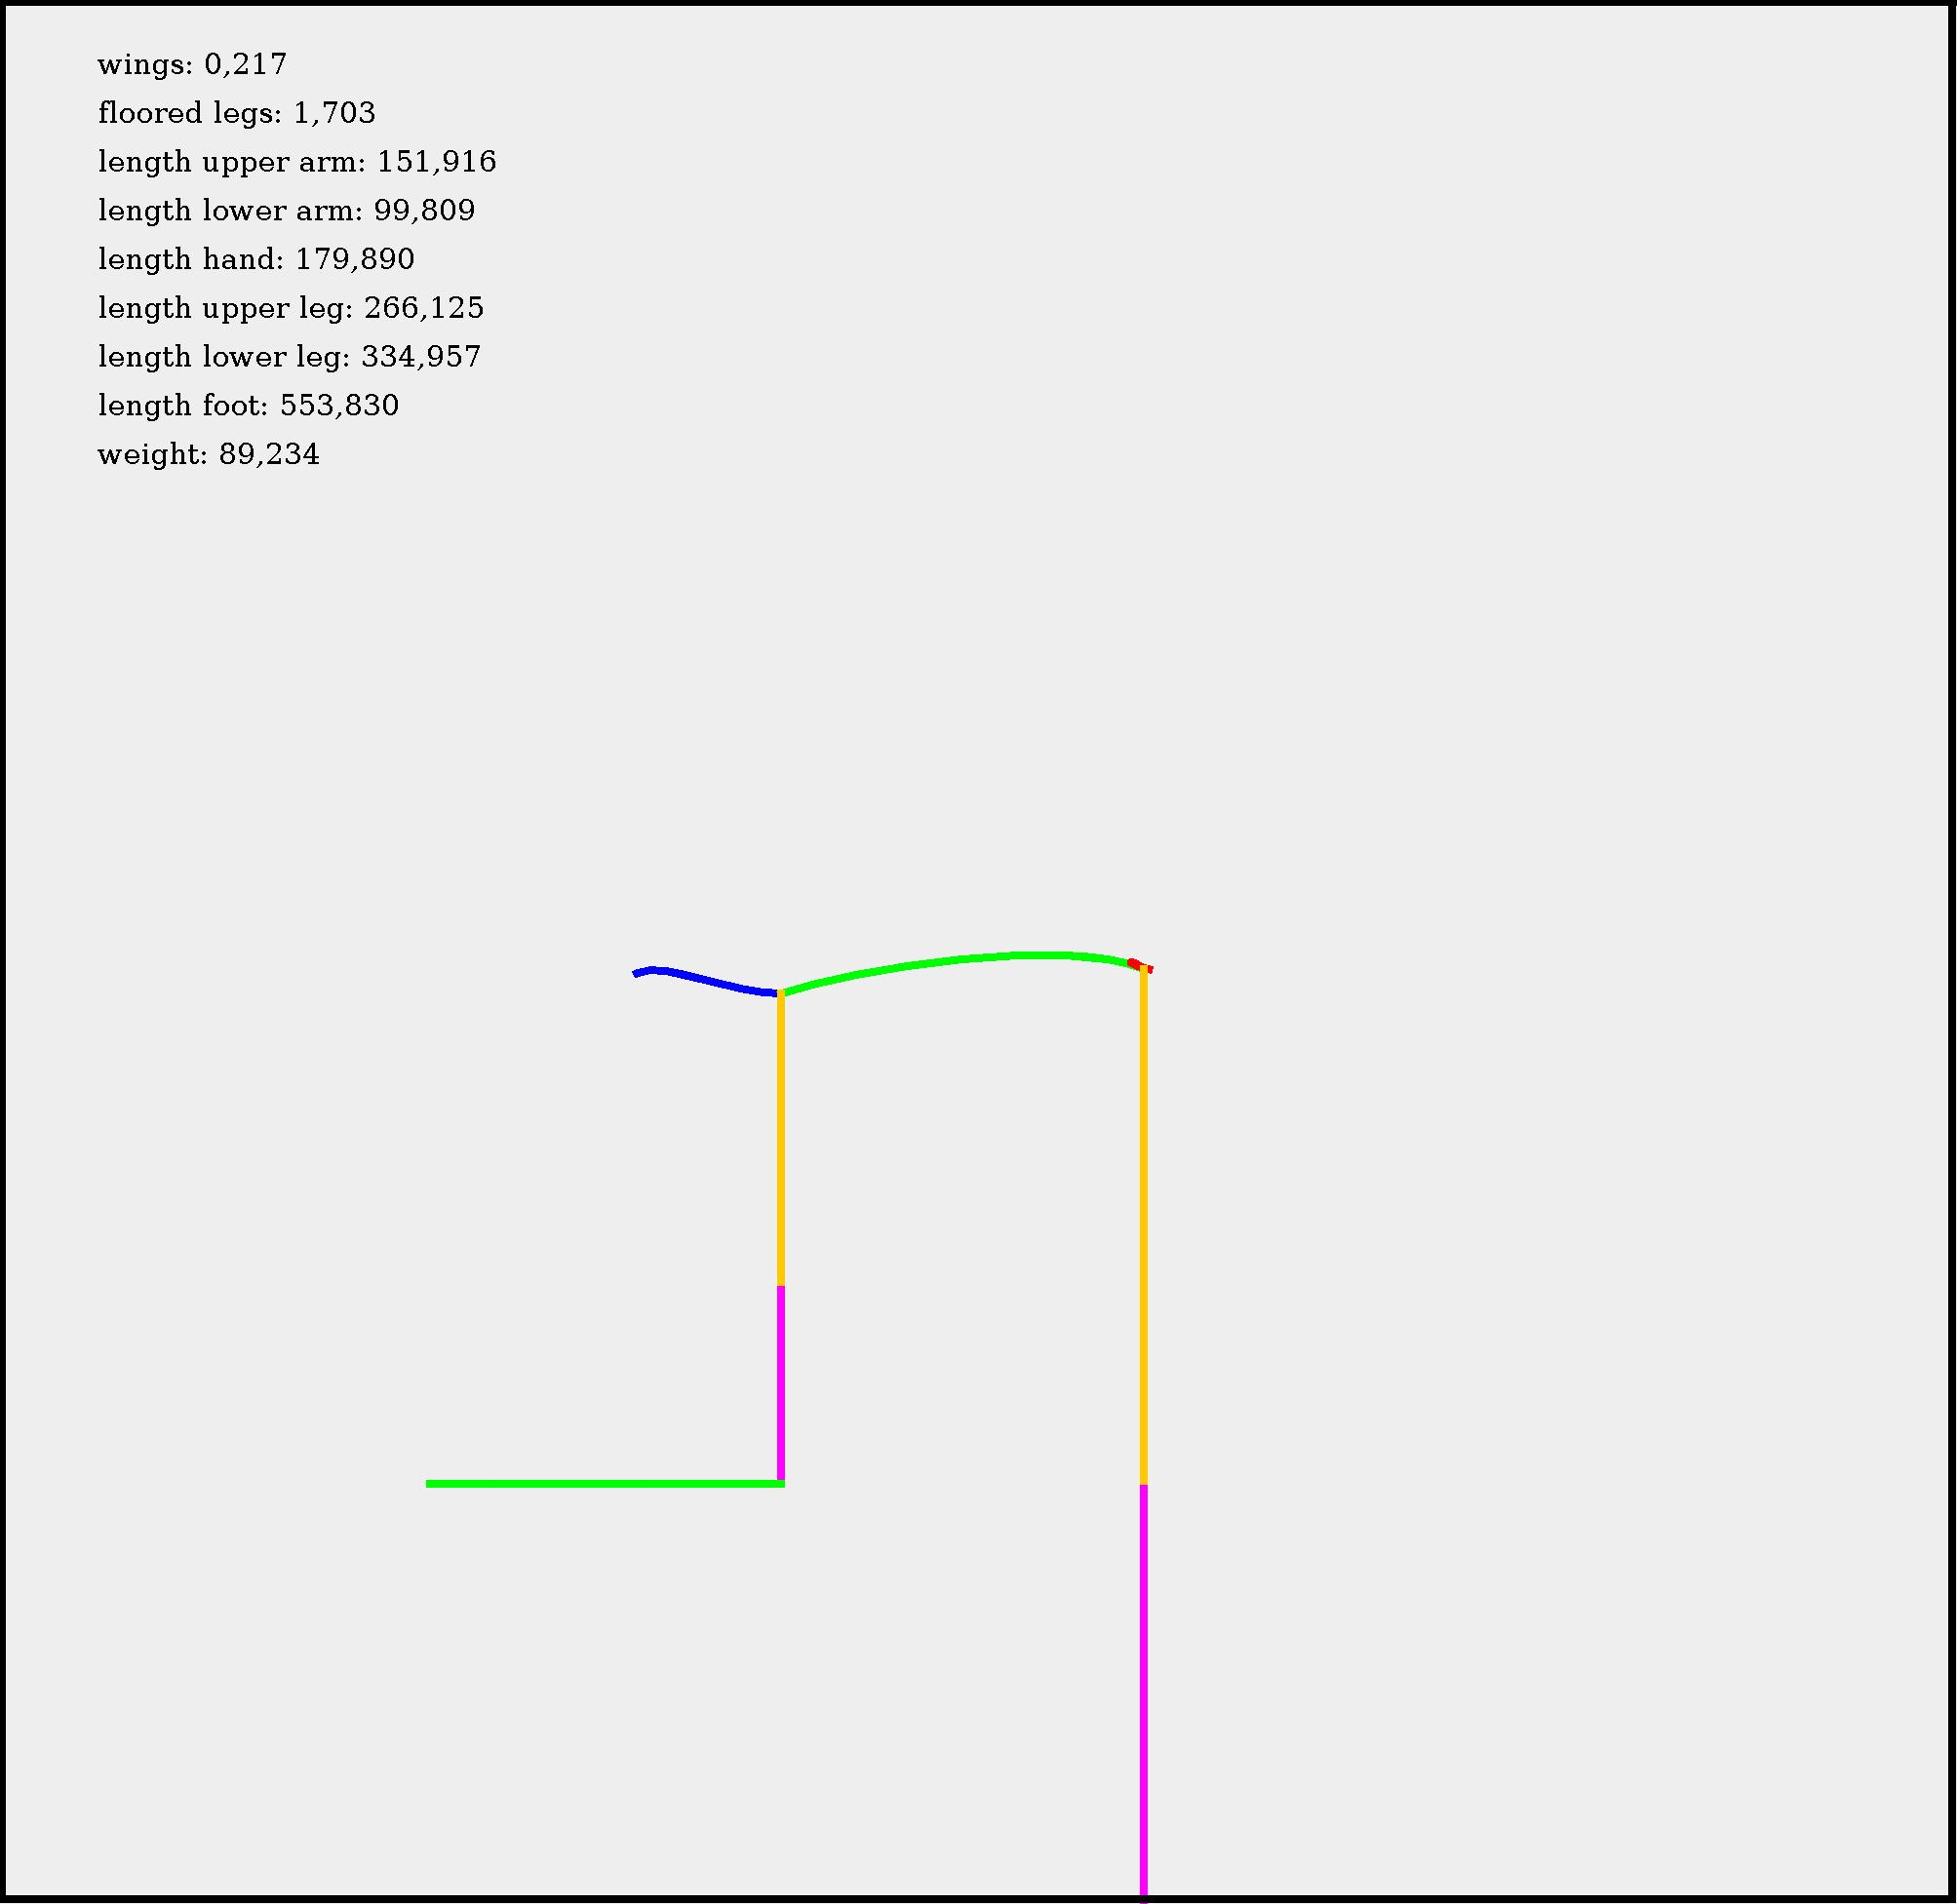
\includegraphics[width=0.4\textwidth]{../PCA/animal_reconstructions_log_weight_downscaled_wings_legs_and_weight/20EV/Frosch_Ausschnitt.jpg}}
  \qquad
  \subfloat[Eingabebild]{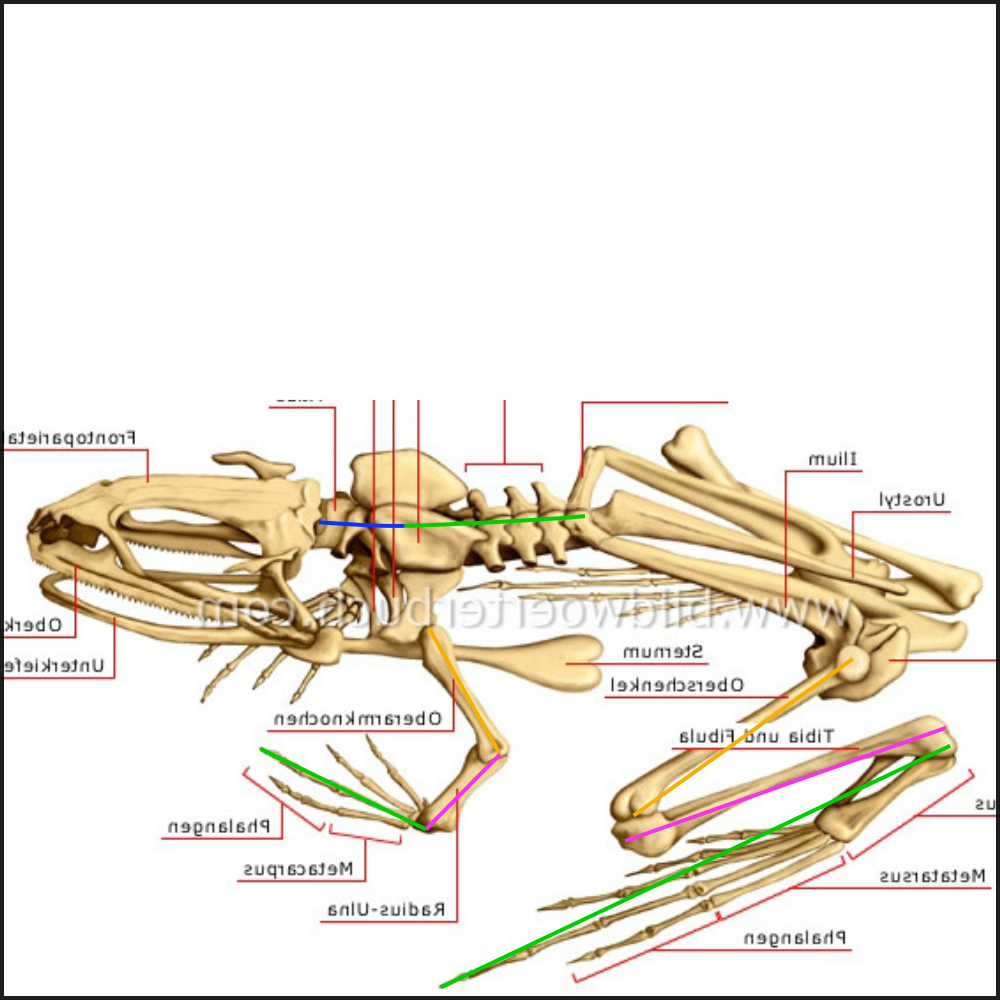
\includegraphics[width=0.4\textwidth]{../PCA/Skelettbilder/Frosch_farbig.png}}
  
  \caption{Frosch, Rekonstruktionen aus den größten $6$, $10$ und $20$ Eigenvektoren und das Eingabebild (d). Der Originalwert für das \emph{Gewicht} ist $0{,}01$kg.}
  \label{frosch}
 \end{figure}
 
 
 Um zu verstehen in welchem Bereich sich die zufällig generierten Punkte bewegen, ist es sinnvoll sich anzuschauen was die Hauptkomponenten "`bedeuten"'. In Abbildung \ref{pca_results_sqrtEV_biggest} sind zwei Datenpunkte zu sehen, die auf der Koordinatenachse liegen, die zum Eigenvektor mit dem größten Eigenwert gehört. Ihr Wert in dieser Dimension ist jeweils die positive \bzw negative Standardabweichung. Die Varianz entlang eines Eigenvektors ist gegeben durch den Eigenwert. Die Standardabweichung ist also die Wurzel des entsprechenden Eigenwerts. Es ist zu sehen wie sich die Punkte verändern, wenn sie sich entlang dieser Achse bewegen \bzw welchen Einfluss der Eigenvektor ausübt.\\
 Die Abbildung \ref{pca_results_sqrtEV_biggest} zeigt, dass der Eigenvektor zum größten Eigenwert einen großen Einfluss auf die Halswirbelsäule hat. Bestätigt wird dies dadurch, dass die größten Einträge des Eigenvektors die $y$-Koordinaten des ersten, zweiten und dritten Kontrollpunkts der Bézierkurve der Halswirbelsäule sind.\\
 Abbildungen nach dem gleichen Schema für die sechs größten Eigenvektoren sind im Anhang in Abbildung \ref{pca_results_sqrtEV} zu finden.
 
 \begin{figure}[h]
   \subfloat[$-\sigma$, \emph{Flügel} $0{,}38$, \emph{Beine mit Bodenkontakt} $1{,}6$, \mbox{\emph{Gewicht} $92$kg}]{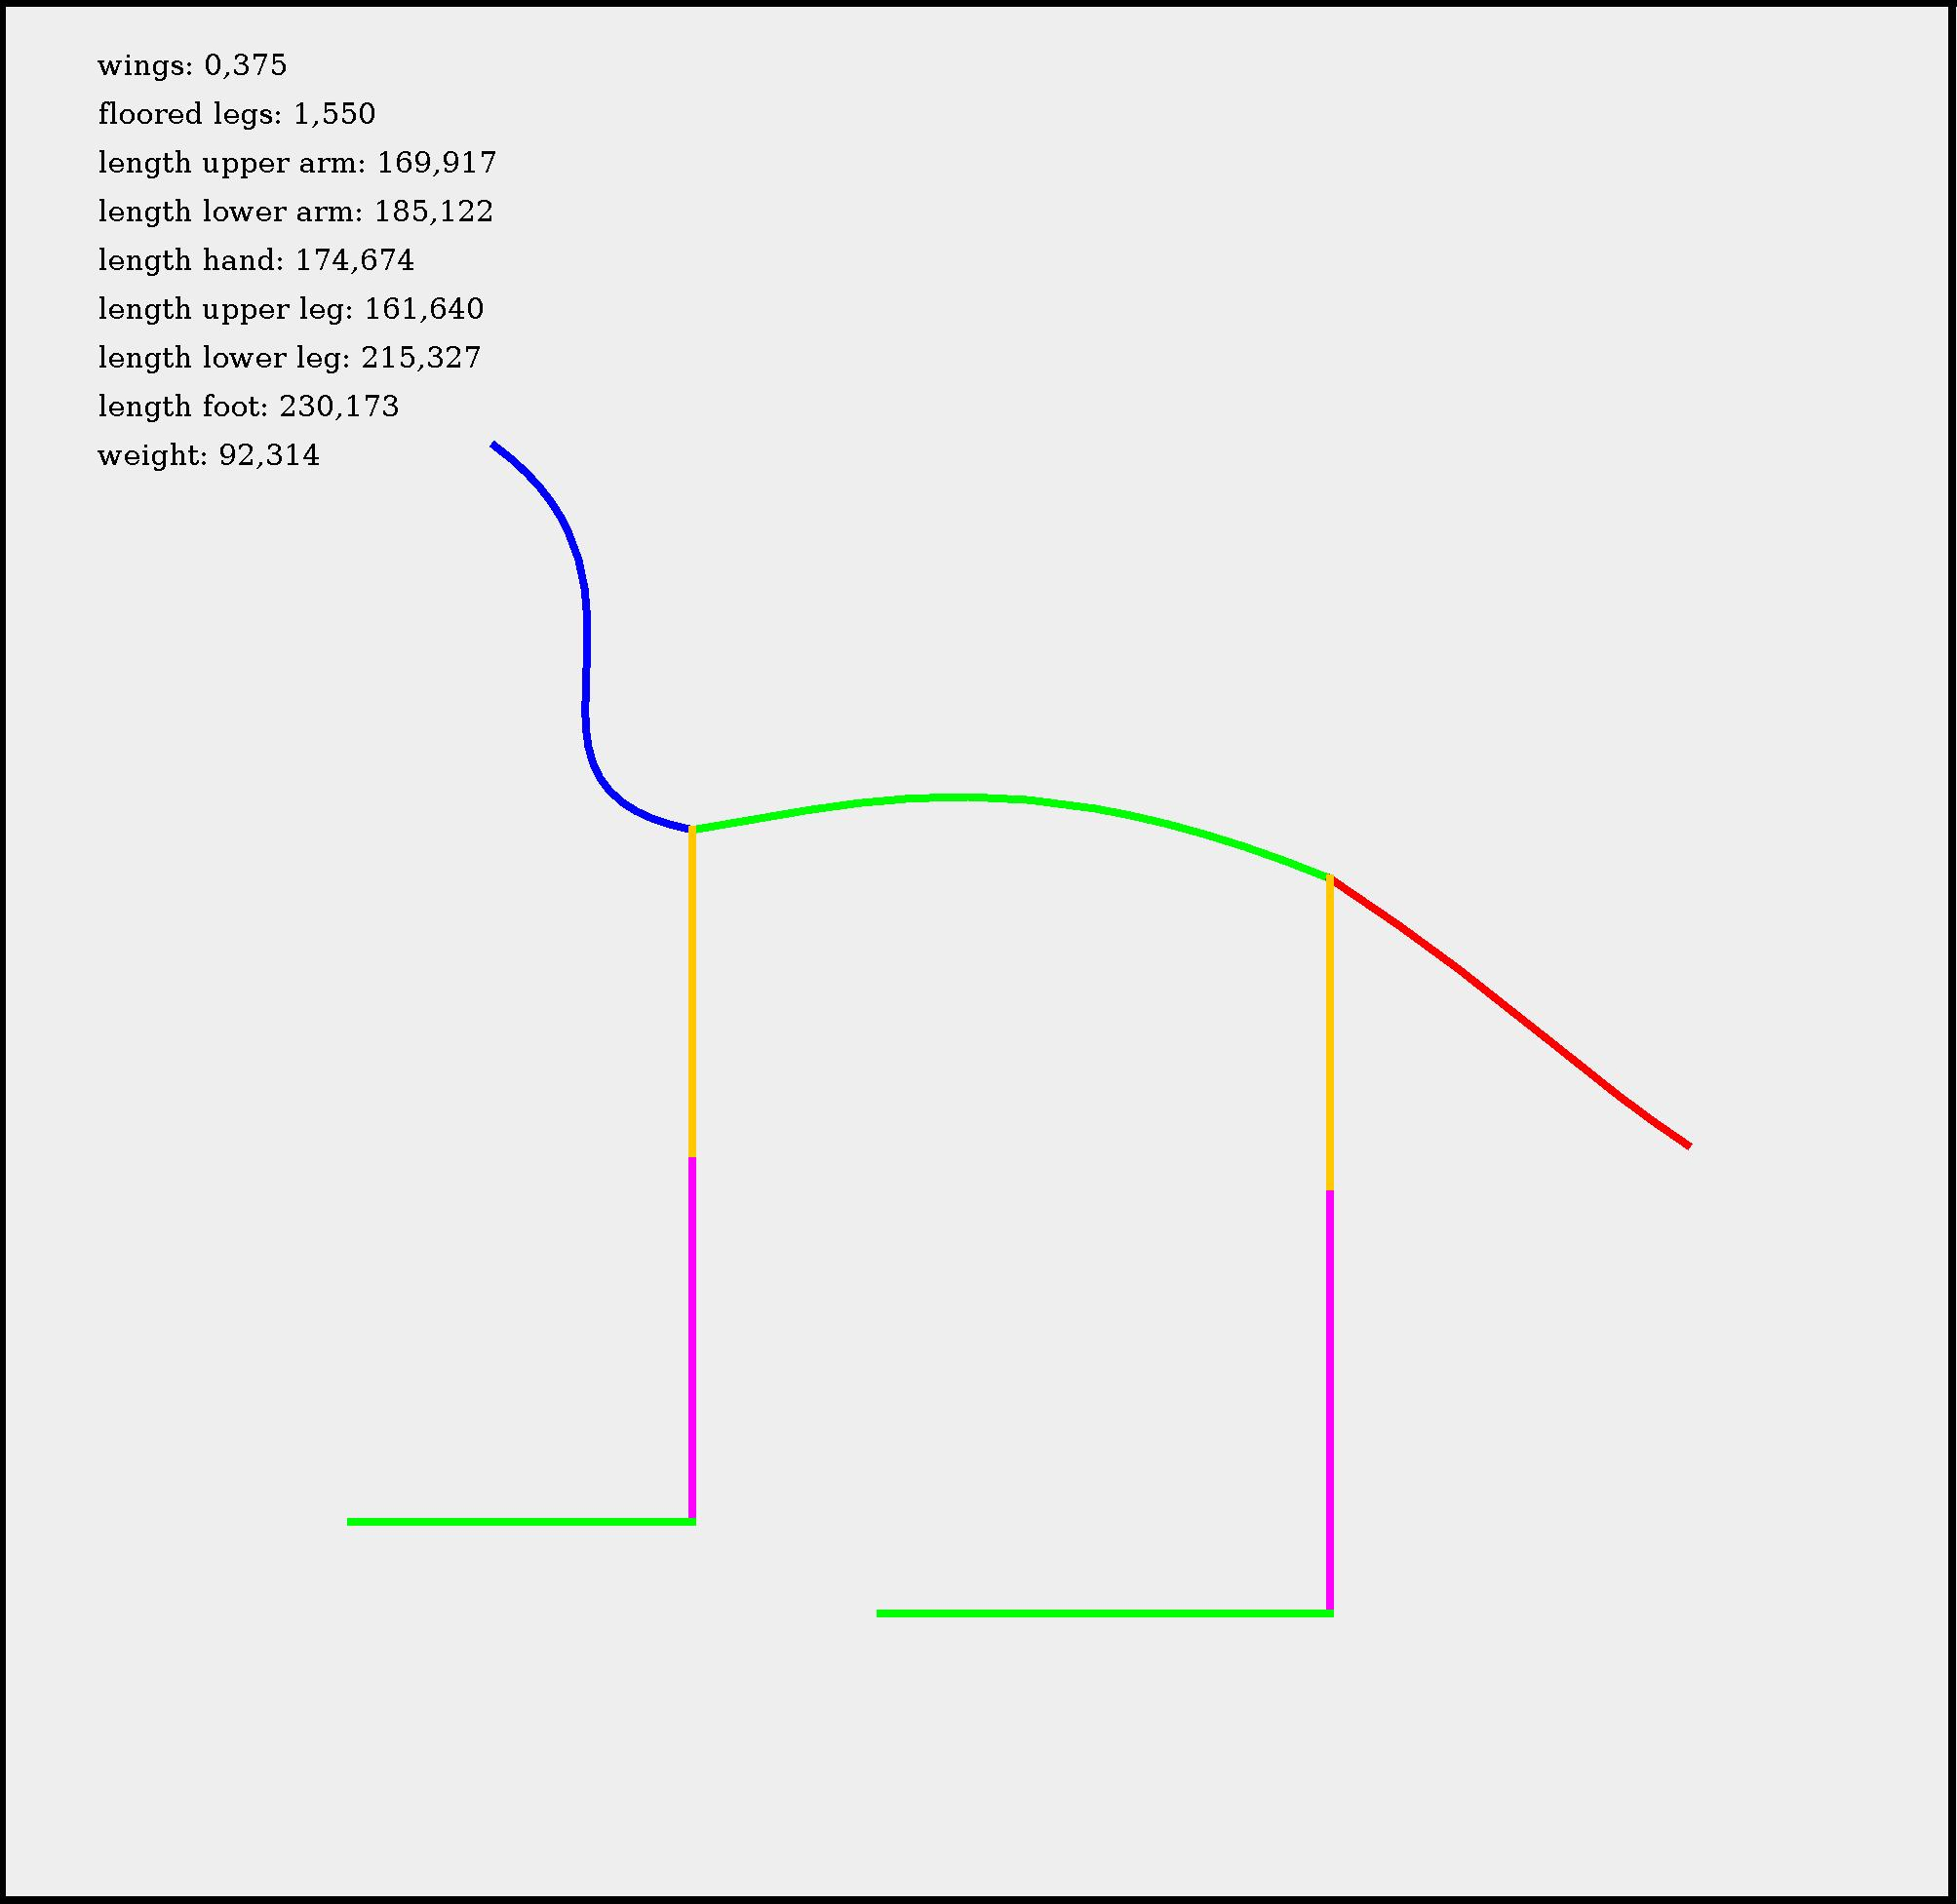
\includegraphics[width=0.5\textwidth]{../PCA/sqrtEV_log_weight_downscaled_wings_legs_and_weight/EV1_neg.jpg}}
   \qquad
   \subfloat[$+\sigma$, \emph{Flügel} $-0{,}057$, \emph{Beine mit Bodenkontakt} $1{,}2$, \mbox{\emph{Gewicht} $94$kg}]{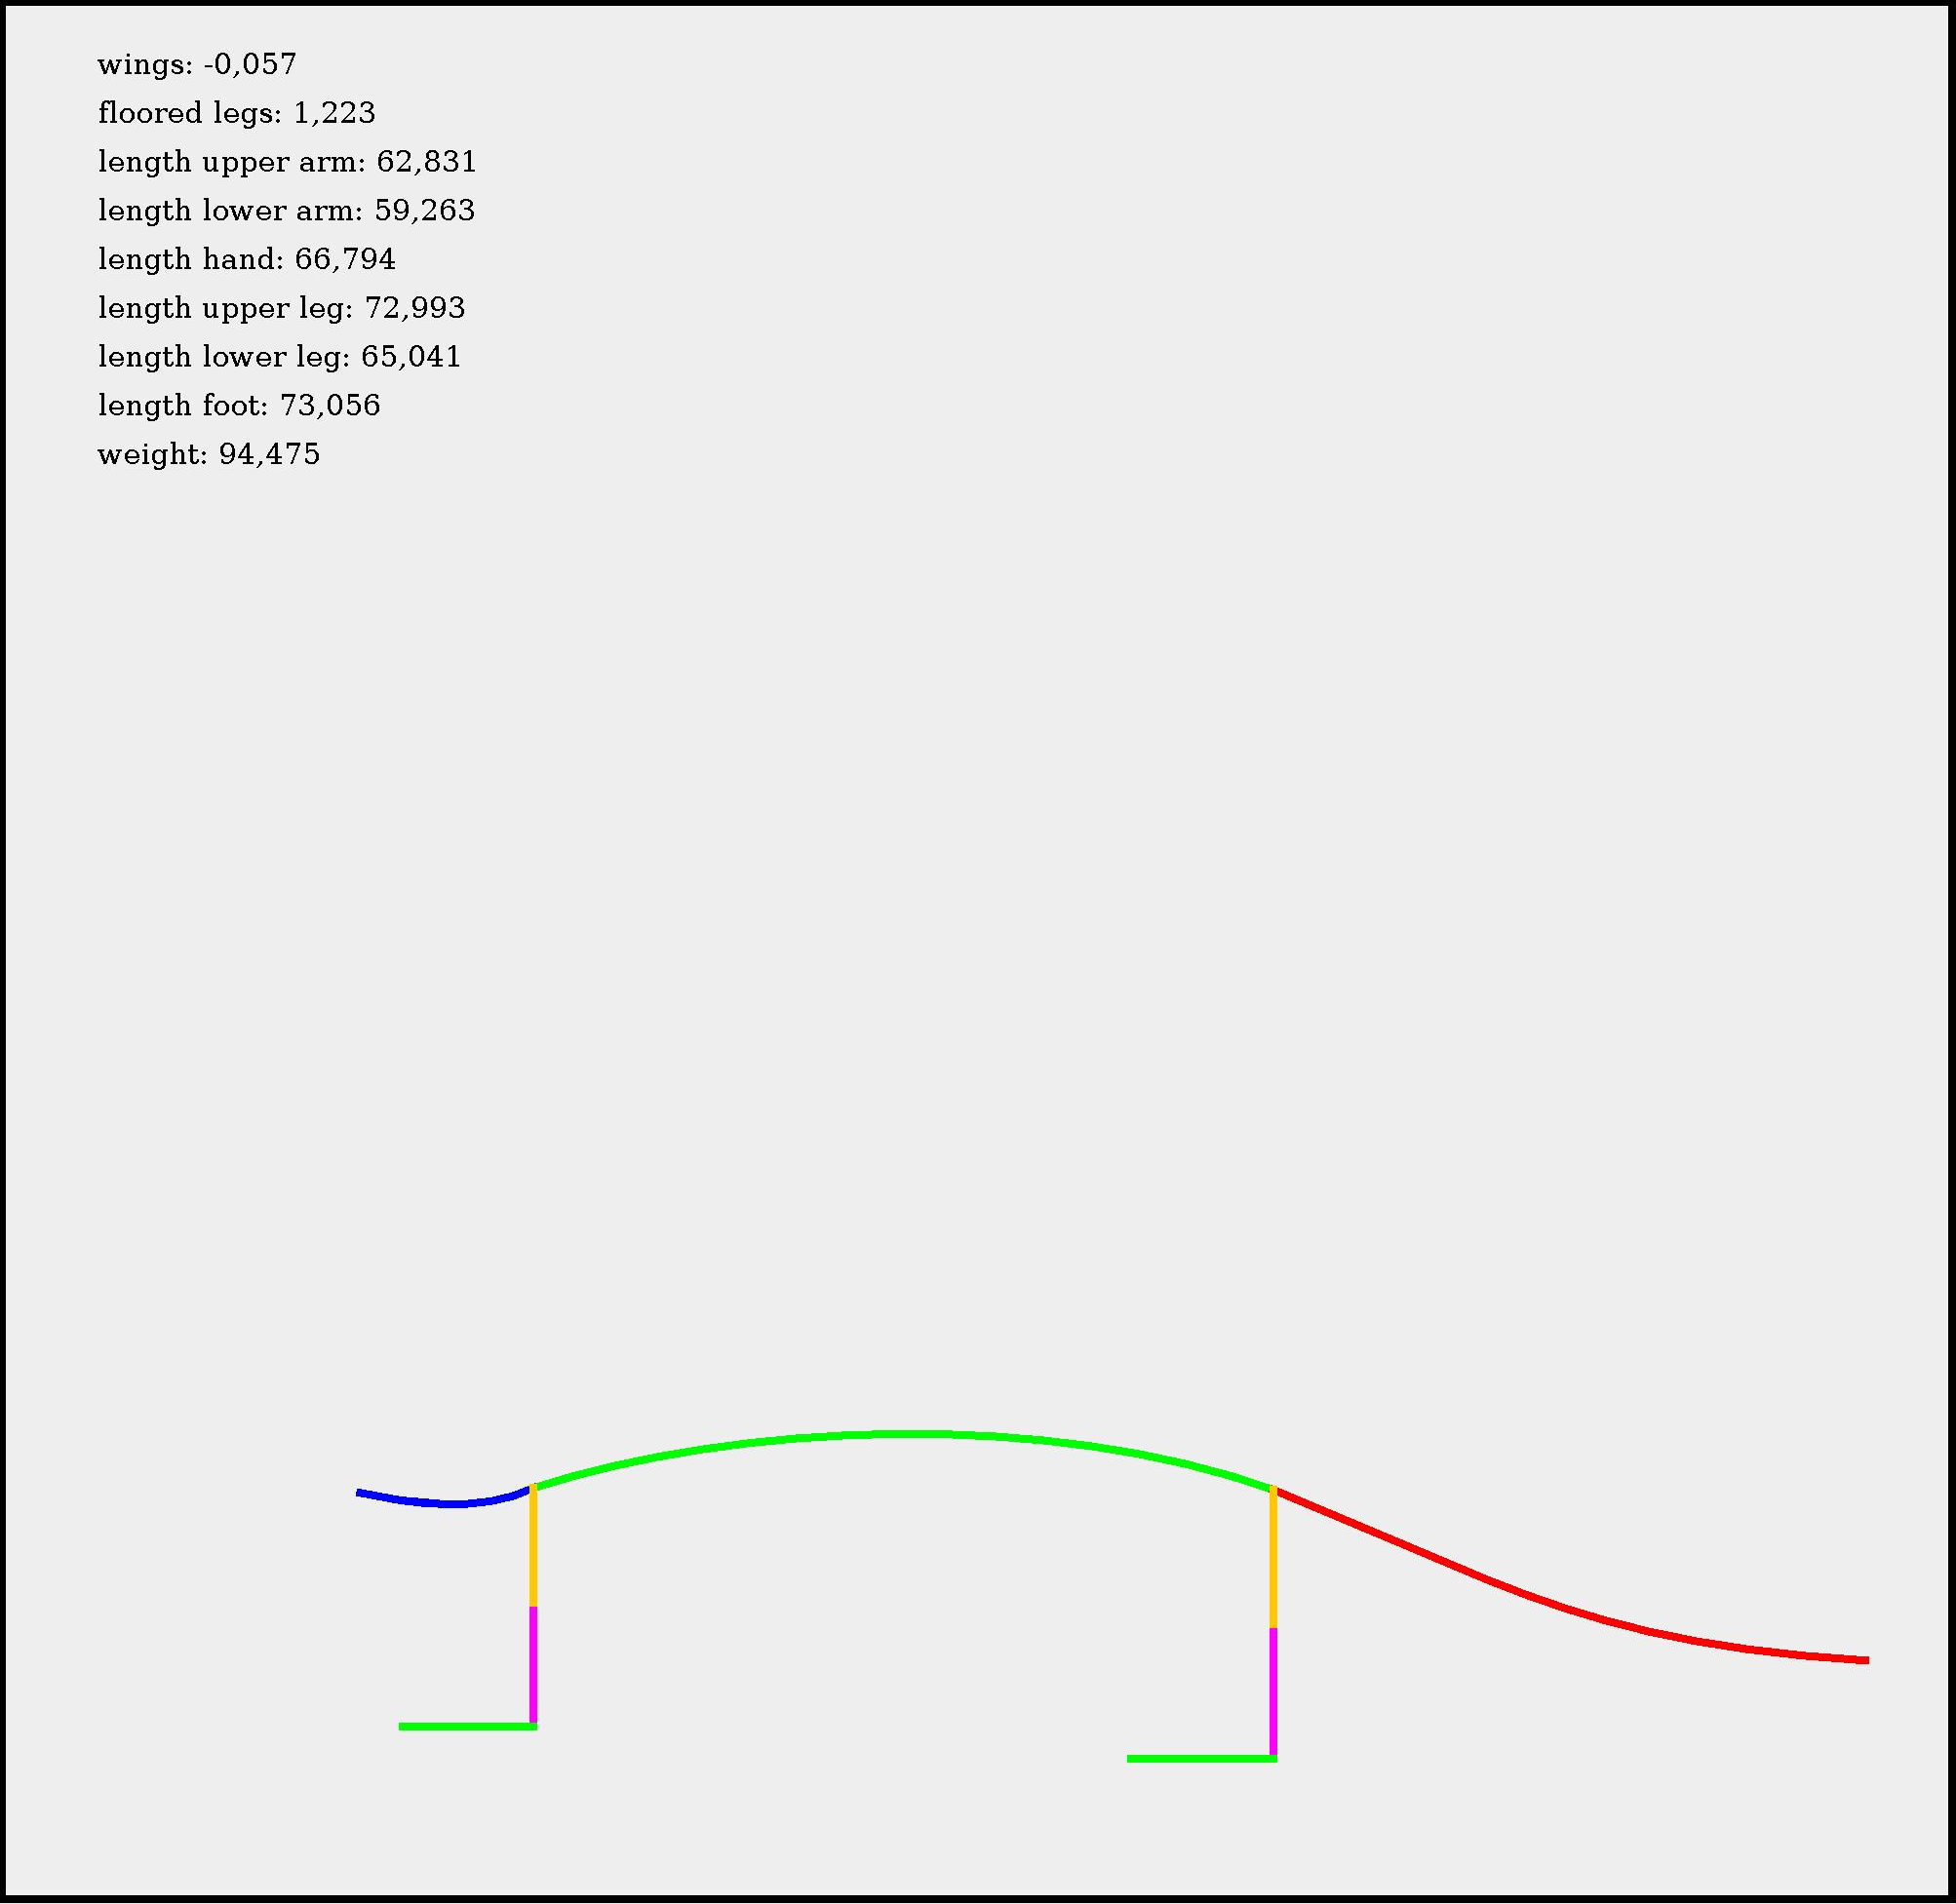
\includegraphics[width=0.5\textwidth]{../PCA/sqrtEV_log_weight_downscaled_wings_legs_and_weight/EV1_pos.jpg}}
   
   \caption{Datenpunkte im PCA-Koordinatensystem. Die Koordinate für den Eigenvektor zum größten Eigenwert nimmt den Wert der positiven \bzw negativen \mbox{Standardabweichung $\sigma$} an, alle anderen sind null. Für Abbildungen zu den größten sechs Eigenvektoren siehe Abbildung \ref{pca_results_sqrtEV} im Anhang}
   \label{pca_results_sqrtEV_biggest}
 \end{figure}

 \paragraph{Auswirkungen von Veränderungen auf den Eingabedaten}
 Bei allen Eingabedimension, außer der Position der Wirbelsäule, kann man die Frage stellen, ob sie nötig sind, oder ob sie die Ergebnisse der PCA eher verschlechtern. Deshalb wurden versuchsweise verschiedene (Kombinationen von) Merkmalen weggelassen. Die Ergebnisse unterscheiden sich aber kaum von der PCA mit allen Daten. \\
 Leider gibt es keine gute Möglichkeit die Qualität der Ergebnisse der PCA zu messen. Man könnte den Unterschied zwischen den Eingabedaten und den Rekonstruktionen aus den Linearkombinationen der Eigenvektoren mit den größten Eigenwerten messen. Da aber verschiedene Dimensionen fehlen, ist nicht klar wie dieser Unterschied einheitlich gemessen werden soll.
 Jedes Merkmal, das nicht verworfen wird, liefert dem Algorithmus, der später Skelette generieren soll, mehr Informationen. Deshalb wurde kein Merkmal verworfen.
 
 Außerdem gibt es die Möglichkeit die Eingabedaten in mehrere Mengen aufzuteilen und diese einzeln zu analysieren. Hierbei gibt es zunächst das Problem, dass sich dann die Anzahl der Datenpunkte noch weiter reduziert, was die Ergebnisse nicht mehr repräsentativ macht.\\
 Merkmale, die sich zur Unterteilung in Mengen anbieten würden, sind die diskreten, also \emph{Flügel} und \emph{Beine mit Bodenkontakt}. Sie sind auch klar als Cluster im Koordinatensystem der PCA ohne angepasste Skalierung zu erkennen (Abbildung \ref{projections_scales} a).
 Getestet wurde die Aufteilung anhand der Werte für die Flügel, da sich dadurch nur zwei Gruppen ergeben. Tatsächlich liefert sie bessere Rekonstruktionen aus den größten Eigenvektoren. Das liegt aber natürlich in erster Linie daran, dass die zu untersuchende Datenmenge jeweils verkleinert wurde.
 
 Ein weiteres Problem daran, die Daten in mehrere Mengen aufzuteilen, ist, dass dann keine Skelette mehr erzeugt werden können, die zwischen den beiden Gruppen liegen. Tatsächlich sehen die Datenpunkte, die zwischen den Gruppen erzeugt werden, aber relativ sinnvoll aus (siehe Abbildung \ref{between_clusters}).
 Auch das ist ein Argument dafür keine Aufteilung vorzunehmen.
 
 \begin{figure}[H]
  \centering
  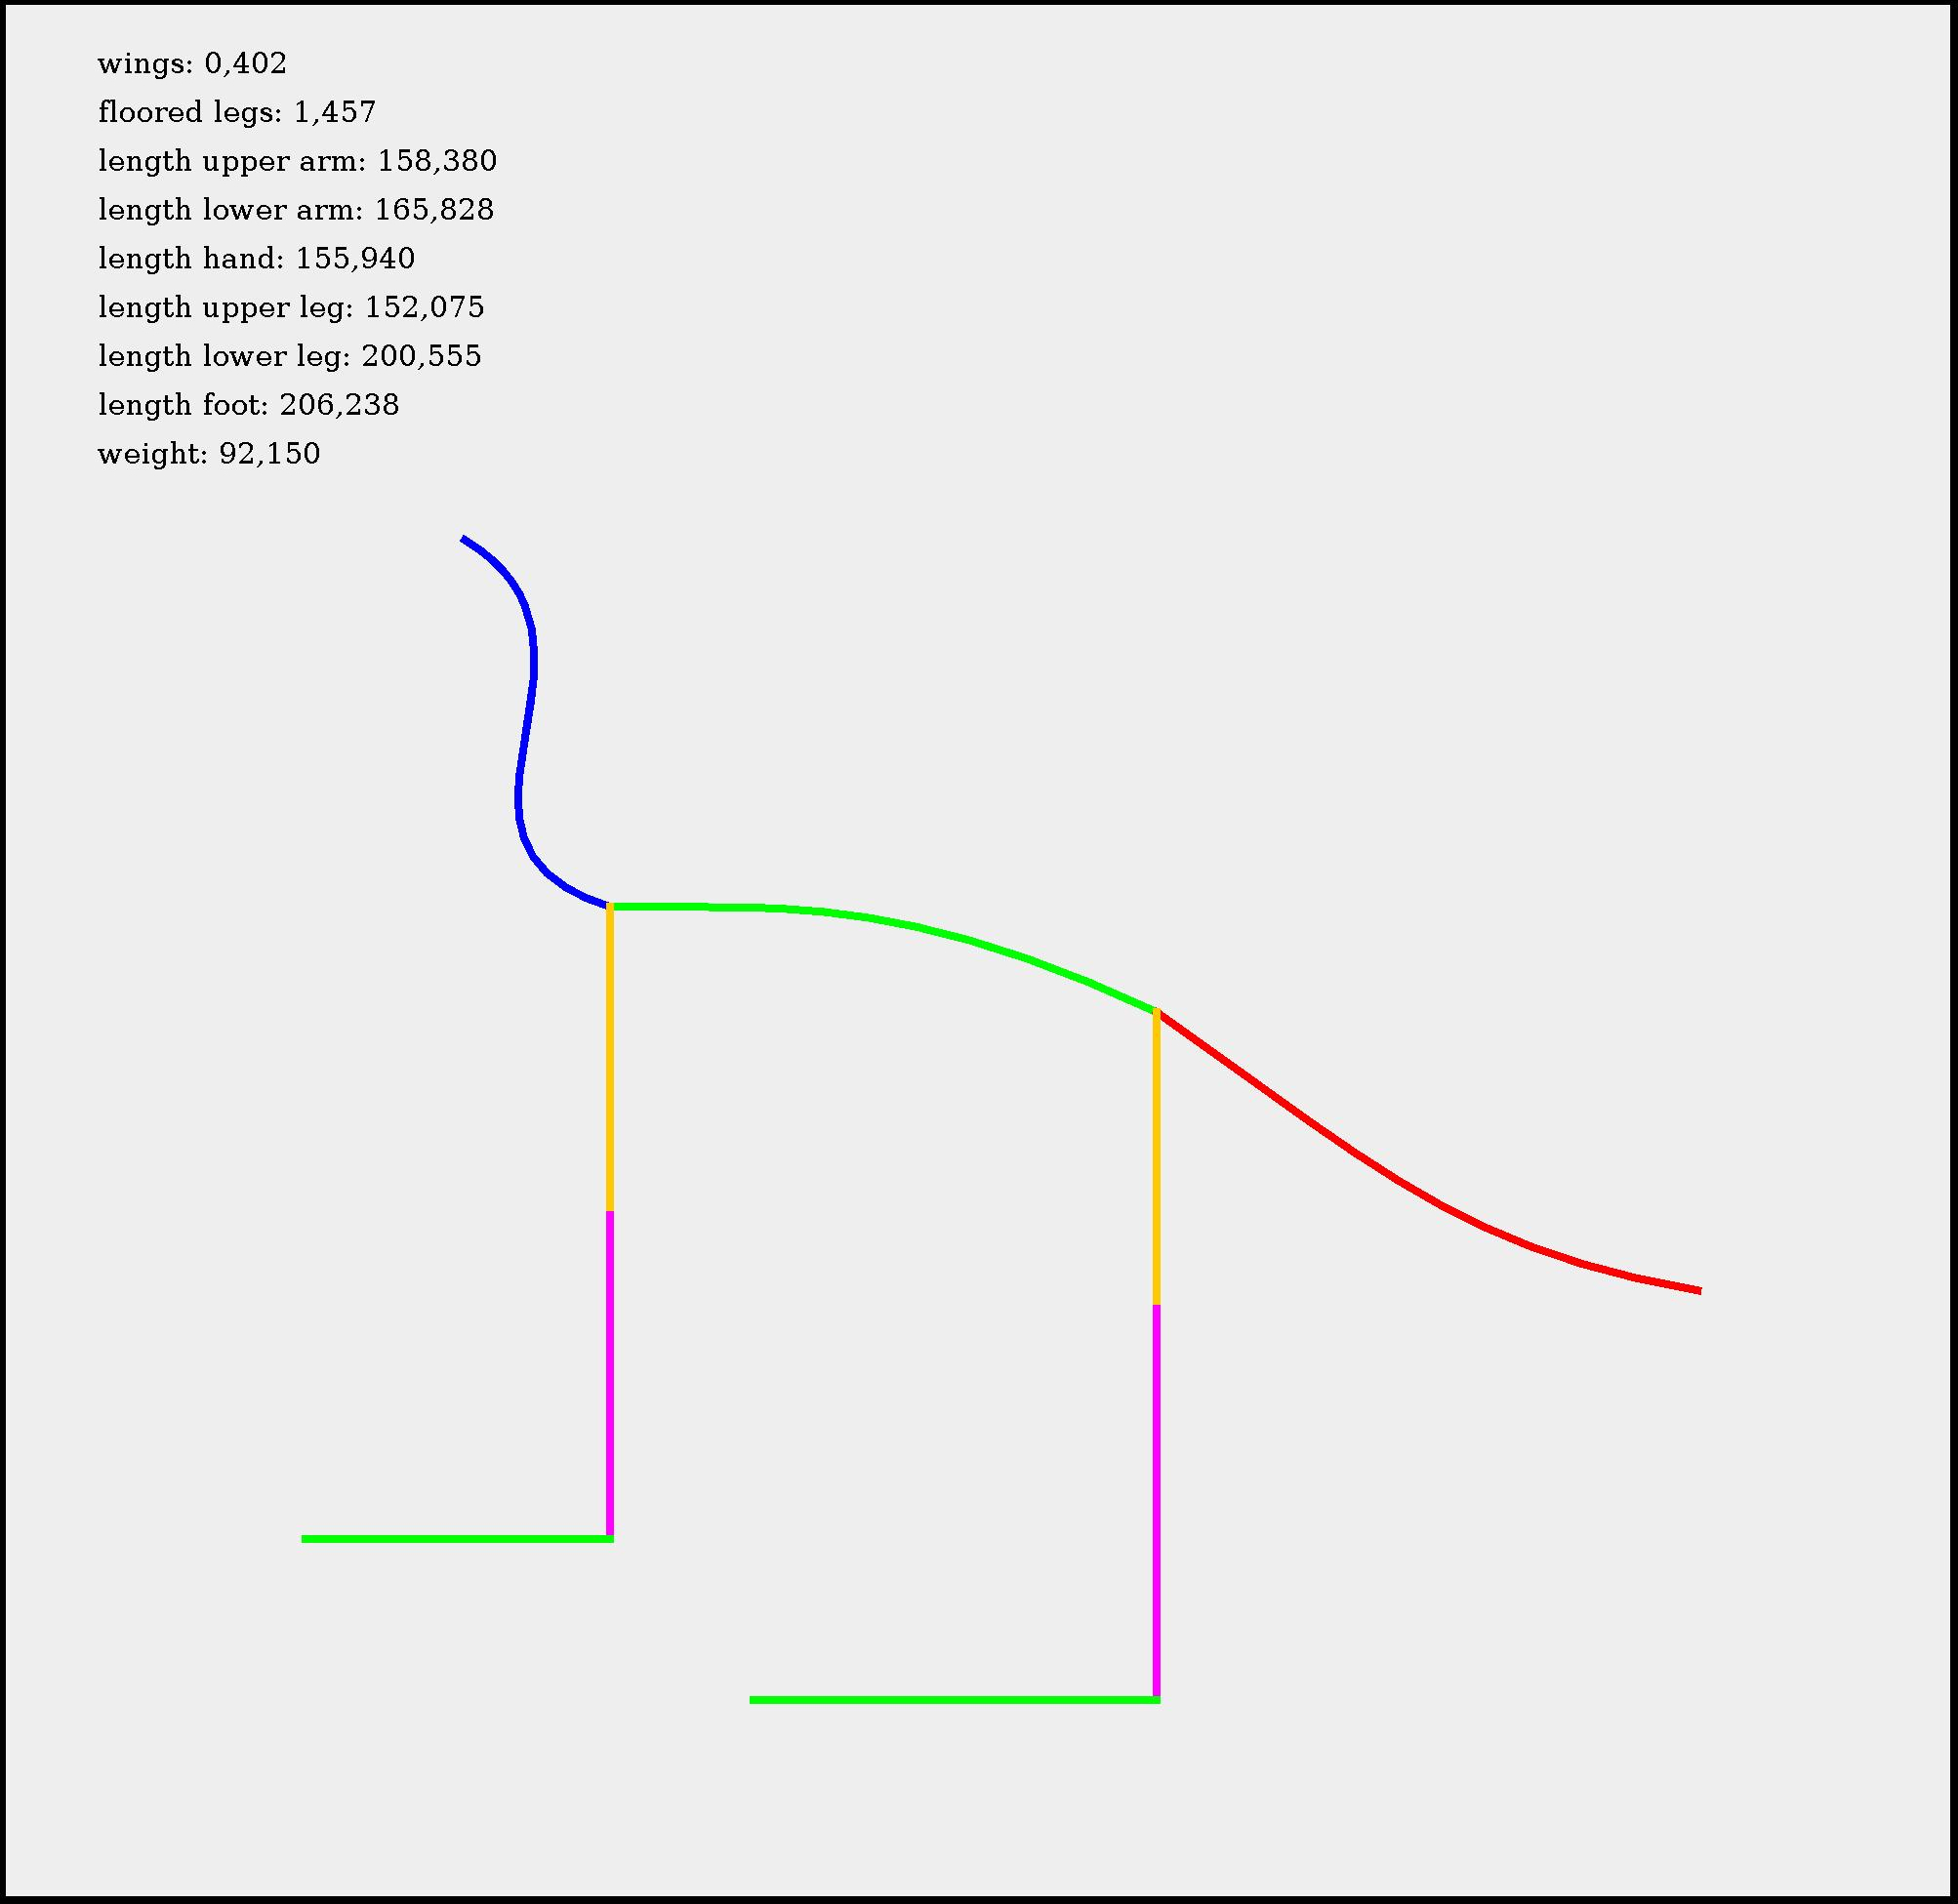
\includegraphics[width=0.5\textwidth]{graphics/betweenClusters.jpg}
  \caption{Visualisierung eines Punktes, der, projiziert auf die ersten beiden Eigenvektoren, zwischen den Eingabedaten mit Flügeln und jenen ohne Flügel liegt. Die Werte, die auf den jeweiligen Achsen angenommen werden, sind $-0{,}4$ für den ersten Eigenvektor und $0{,}2$ für den zweiten. Werte für die ursprünglichen Merkmale, die nicht visualisiert sind, sind folgende: \emph{Flügel} $0{,}402$, \emph{Beine mit Bodenkontakt} $1{,}46$ und \emph{Gewicht} $92{,}2$kg.}
  \label{between_clusters}
 \end{figure}

 
 \newpage
 %-------------------------------------------------
 \section{Bedingte Verteilungen}
 \label{pca_conditions}
 
 Aus den Ergebnissen der PCA lassen sich sehr gut zufällige Skelette erzeugen. Es ist aber schwer gezielt Eigenschaften festzulegen.
 
 \paragraph{Bedingungen an explizit erhobene Merkmale}
 Der erste Schritt dies zu erreichen ist, Eigenschaften, die so schon in den erhobenen Daten vorkommen, auf spezifische Werte festzulegen. Das können beispielsweise die Anzahl der Beine sein oder ob das Skelett Flügel haben soll.
 
 Dazu kann man, statt die ursprünglichen Daten und deren Verteilung zu verwenden, die entsprechenden bedingten Verteilungen bilden. Dazu muss der bedingte Mittelwert und die bedingte Kovarianzmatrix, wie in \cite[S.\ $116$ f.]{conditionalDistribution} beschrieben, bestimmt werden.
 
 Seien 
 \[x = \begin{pmatrix} x_1 \\ x_2 \end{pmatrix}, 
  \mu = \begin{pmatrix} \mu_1 \\ \mu_2 \end{pmatrix} \text{ und }
  \Sigma = \begin{pmatrix} \Sigma_{11} & \Sigma_{12} \\ \Sigma_{21} & \Sigma_{22} \end{pmatrix}. \] 
 
 Der Zufallsvektor $x$ enthält $n$ normalverteilte Zufallsvariablen, $q \le n$ Variablen im \mbox{Vektor $x_1$} und $n - q$ in $x_2$. Die Einträge in $\mu$ sind die jeweils zugehörigen Mittelwerte und $\Sigma$ ist die Kovarianzmatrix. Die Verteilung für $x_1$ unter der Bedingung, dass $x_2 = b$, hat den \mbox{Mittelwert $\bar{\mu}$} und Kovarianzmatrix $\overline{\Sigma}$ mit
 
 \[ \bar{\mu} = \mu_1 + \Sigma_{12}~ \Sigma_{22}^{-1}~ (b - \mu_2), \quad
    \overline{\Sigma} = \Sigma_{11} - \Sigma_{12}~ \Sigma_{12}^{-1}~ \Sigma_{21}. \]
 
 Verwendet man nun $\overline{\Sigma}$ als Eingabe für die PCA, so erhält man nur noch Daten für Skelette unter den vorher festgelegten Bedingungen $b$. Zu beachten ist hier, dass die Eigenvektoren sich im Vergleich zur PCA ohne Bedingungen verändern. Falls man diese also zur Bestimmung eines Datenpunktes verwendet hat (\zb in einer Benutzeroberfläche), so müssen die Werte für die neuen Eigenvektoren neu ausgerechnet werden.
 
 % feste Werte variieren
 Erzeugt man nun in diesem bedingten Raum zufällige Beispiele, zeigt sich sehr deutlich, dass das Festlegen von nur einer Dimension auch die anderen Dimensionen stark einschränken kann. Legt man \zb fest, dass das Skelett keine Flügel haben soll, so sind sich die Wirbelsäulen der Skelette, die dann bedingt zufällig generiert werden, sehr ähnlich (siehe Abbildung \ref{spine_variance}a).\\
 Um das zu umgehen, wird die Eingabe als Intervall aufgefasst, aus dem zufällig ein Wert gezogen wird. Legt der Benutzer \zb einen ganzzahligen Wert fest, so wird ein kleiner zufälliger Wert aufaddiert oder abgezogen. So wird nicht immer genau der gleiche Wert verwendet. Zwei Beispiele sind in den Abbildungen \ref{spine_variance} b und c gezeigt. Zusätzlich ist dieses Vorgehen hilfreich, weil dann vom Benutzer nicht verlangt wird Bedingungen für \emph{Flügel} oder \emph{Beine} anzugeben, die nicht ganzzahlig sind, um mehr Variation zu bekommen. 
 
 \begin{figure}
  \subfloat[$0$ Flügel, ohne Anpassung]{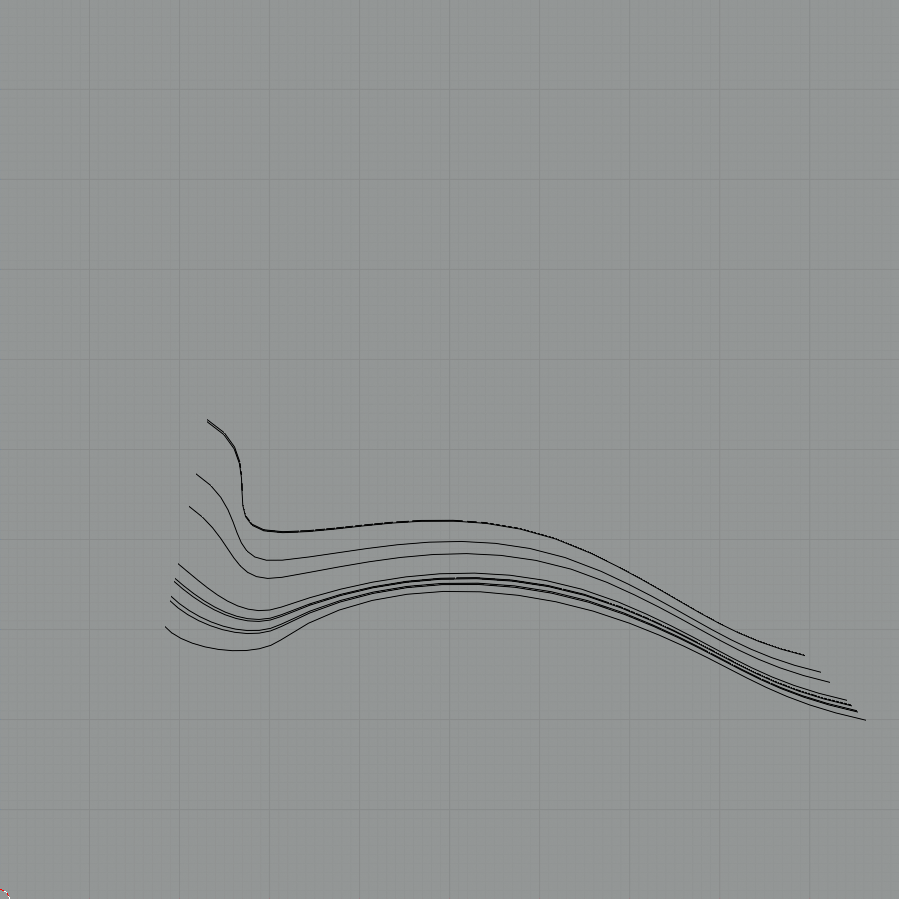
\includegraphics[width=0.3\textwidth]{graphics/0wings_withoutAdditionalVariance.png}}
  \qquad
  \subfloat[$0$ Flügel, mit Anpassung]{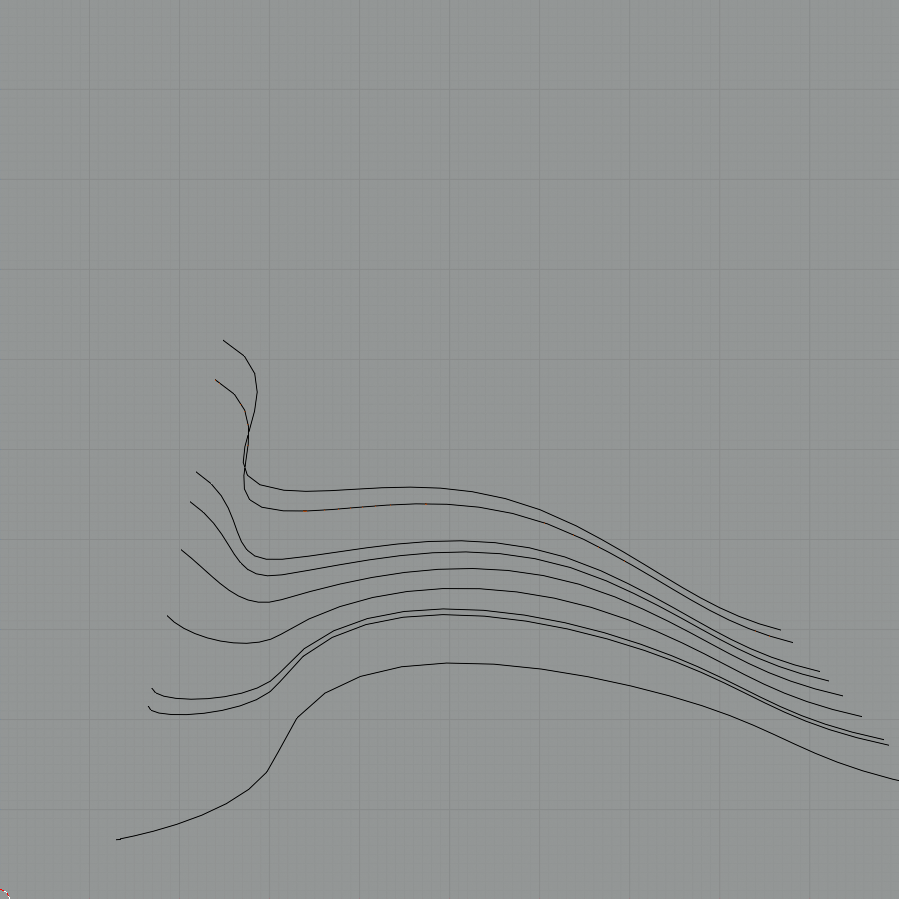
\includegraphics[width=0.3\textwidth]{graphics/0wings_withAdditionalVariance.png}}
  \qquad
  \subfloat[$1$ Paar Beine, mit Anpassung]{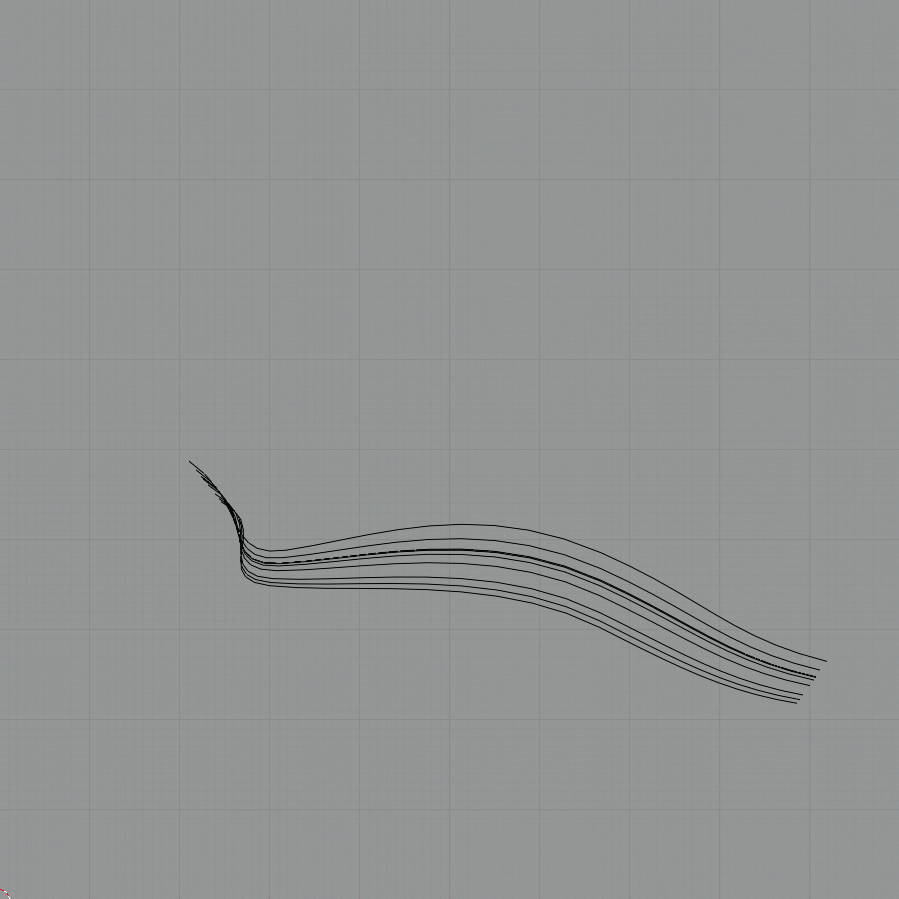
\includegraphics[width=0.3\textwidth]{graphics/1leg_withAdditionalVariance.png}}
  
  \caption{Jeweils $10$ bedingt zufällig generierte Wirbelsäulen. (a) und (b) ohne Flügel, (c) mit einem Paar Beine. In (b) und (c) wird ein zufälliger Wert aus $[-0{,}5, 0{,}5]$ auf die Bedingung (Flügel $= 0$ \bzw Beine $= 1$) aufaddiert.}
  \label{spine_variance}
 \end{figure}

 
 % Übergang Krokodil -> Fisch
 Schaut man sich nun die erzeugten Wirbelsäulen mit einem Paar tragender Beine an (Abbildung \ref{spine_variance}c), so liegen sie alle recht nah an der mittleren Wirbelsäule (Abbildung \ref{mean}).
 Das wirkt zunächst überraschend, da die meisten Tiere in den erhobenen Beispielen, die zwei Beine haben, Vögel sind. Sie haben eine Wirbelsäule, die hoch über dem Boden liegt und relativ aufrecht ist. Dann gibt es noch Känguru und Tyrannosaurus Rex. Bei ihnen liegt die Wirbelsäule ähnlich. Deshalb könnte man eine mittlere Wirbelsäule erwarten, die ebenfalls diese Eigenschaften besitzt.\\
 Es muss aber auch einen Übergang von bodennahen Vierbeinern wie Krokodilen oder Fröschen über Zweibeiner zu Fischen ohne Beine geben, auch wenn es dafür in der Natur eher wenige Beispiele gibt. In den erhobenen Daten sind das nur der Seehund und die Ohrenrobbe. Das ist der Grund, weshalb die mittlere Wirbelsäule für Zweibeiner verhältnismäßig flach verläuft.
 
 \paragraph{Bedingungen an implizit enthaltene Merkmale}
 % Bedingungen an abgeleitet Werte
 Nun möchte man vielleicht Bedingungen an das zu generierende Skelett stellen, die nicht schon genau so in den erhobenen Daten repräsentiert sind. 
 Bedingungen an Dimensionen, die gar nicht erhoben wurden, können  entweder, unabhängig von der PCA, in den Ersetzungsregeln oder den Parametern der Grammatik (siehe Abschnitt \ref{section:grammar}) erzwungen werden, wie \zb die Anzahl der Flossen, oder sie müssen in die Erhebung eingefügt werden.
 
 Bedingungen, die schon implizit in den erhobenen Daten enthalten sind, sind beispielsweise die Schwanz- oder Halslänge. Um an sie Bedingungen stellen zu können, könnte man ebenfalls eine zusätzliche Dimension einfügen. Sie kann einfach aus den schon bestehenden Dimensionen errechnet werden. Dabei wäre aber das Problem, dass nur die Dimensionalität der Daten erhöht wird, nicht aber die eingegebenen Informationen. Es wären also mehr Eingabebeispiele nötig, nur dafür, dass die PCA eine offensichtliche Korrelation der Dimensionen erkennt.
 
 Die bessere Alternative ist die Eingabedimensionen der PCA umzuparametrisieren. Der Abstand vom Anfangs- zum Endpunkt des Schwanzes in x-Richtung, ist \zb implizit in der Differenz der x-Koordinaten des ersten und letzten Kontrollpunktes der Bézierkurve des Schwanzes enthalten. Ersetzt man nun den absoluten x-Wert des letzten Kontrollpunktes durch den Abstand in x-Richtung zum ersten Kontrollpunkt, so lässt sich diese Länge ganz einfach als Bedingung an die PCA stellen. 
 
 % Schwanzlänge messen
 Betrachtet man nun konkret den Wunsch die Schwanzlänge festzulegen, ist das nicht ganz so einfach. Der Abstand vom Anfangs- zum Endpunkt des Schwanzes in x- und y-Richtung lässt sich zwar leicht festlegen, diese Längen sagen aber im Allgemeinen noch nicht viel über die tatsächliche Länge der Bézierkurve aus. Verlangt man \zb eine Länge von $0$px in x-Richtung, so haben die generierten Datenpunkte einen Schwanz der zwar auf gleicher Höhe beginnt und endet, aber trotzdem vorhanden ist und einen kleinen Bogen beschreibt.
 Um die wirkliche Länge des Schwanzes zu messen, müsste man also noch mehr Aufwand in die Umparametrisierung stecken oder doch eine zusätzliche Dimension für die PCA in Kauf nehmen.
 
 
